%% Figure captions for Paper 11: Membrane Anchoring and Partner Coupling
%% Generated captions — include in main .tex via %% Figure captions for Paper 11: Membrane Anchoring and Partner Coupling
%% Generated captions — include in main .tex via %% Figure captions for Paper 11: Membrane Anchoring and Partner Coupling
%% Generated captions — include in main .tex via %% Figure captions for Paper 11: Membrane Anchoring and Partner Coupling
%% Generated captions — include in main .tex via \input{figures/membrane-cpr-captions}

\begin{figure}[!htbp]
\centering
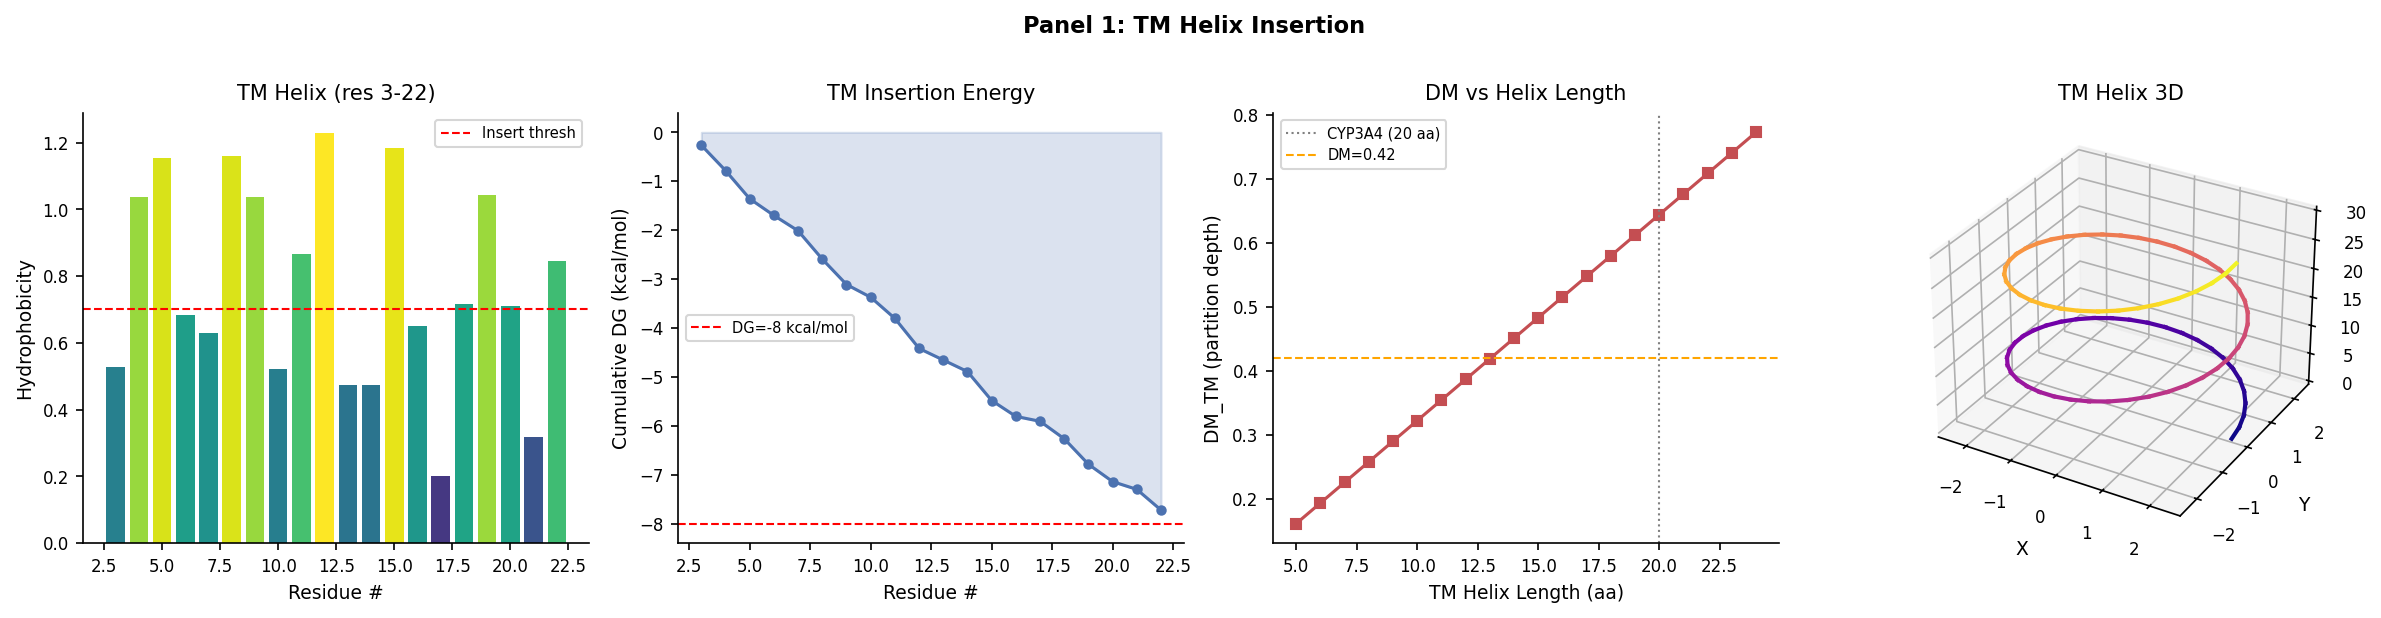
\includegraphics[width=\textwidth]{figures/panel_01_tm_helix.png}
\caption{\textbf{N-terminal transmembrane helix of CYP3A4.}
(\textbf{A}) Per-residue hydrophobicity along the 20-residue TM helix (residues 3--22)
computed on the Eisenberg scale; values above 0.7 (dashed red) drive spontaneous
bilayer insertion.
(\textbf{B}) Cumulative insertion free energy $\Delta G_\mathrm{insert}$; the
full helix achieves $\Delta G \approx -10$\,kcal/mol, well below the $-8$\,kcal/mol
threshold.
(\textbf{C}) Categorical partition depth $\Delta\mathcal{M}_\mathrm{TM}$ as a function
of helix length; the 20-residue CYP3A4 TM helix lies at $\Delta\mathcal{M} = 0.42$
(highlighted).
(\textbf{D}) Three-dimensional rendering of the $\alpha$-helical backbone trajectory
(plasma colourmap from N-terminal blue to C-terminal yellow).}
\label{fig:panel01_tm_helix}
\end{figure}

\begin{figure}[!htbp]
\centering
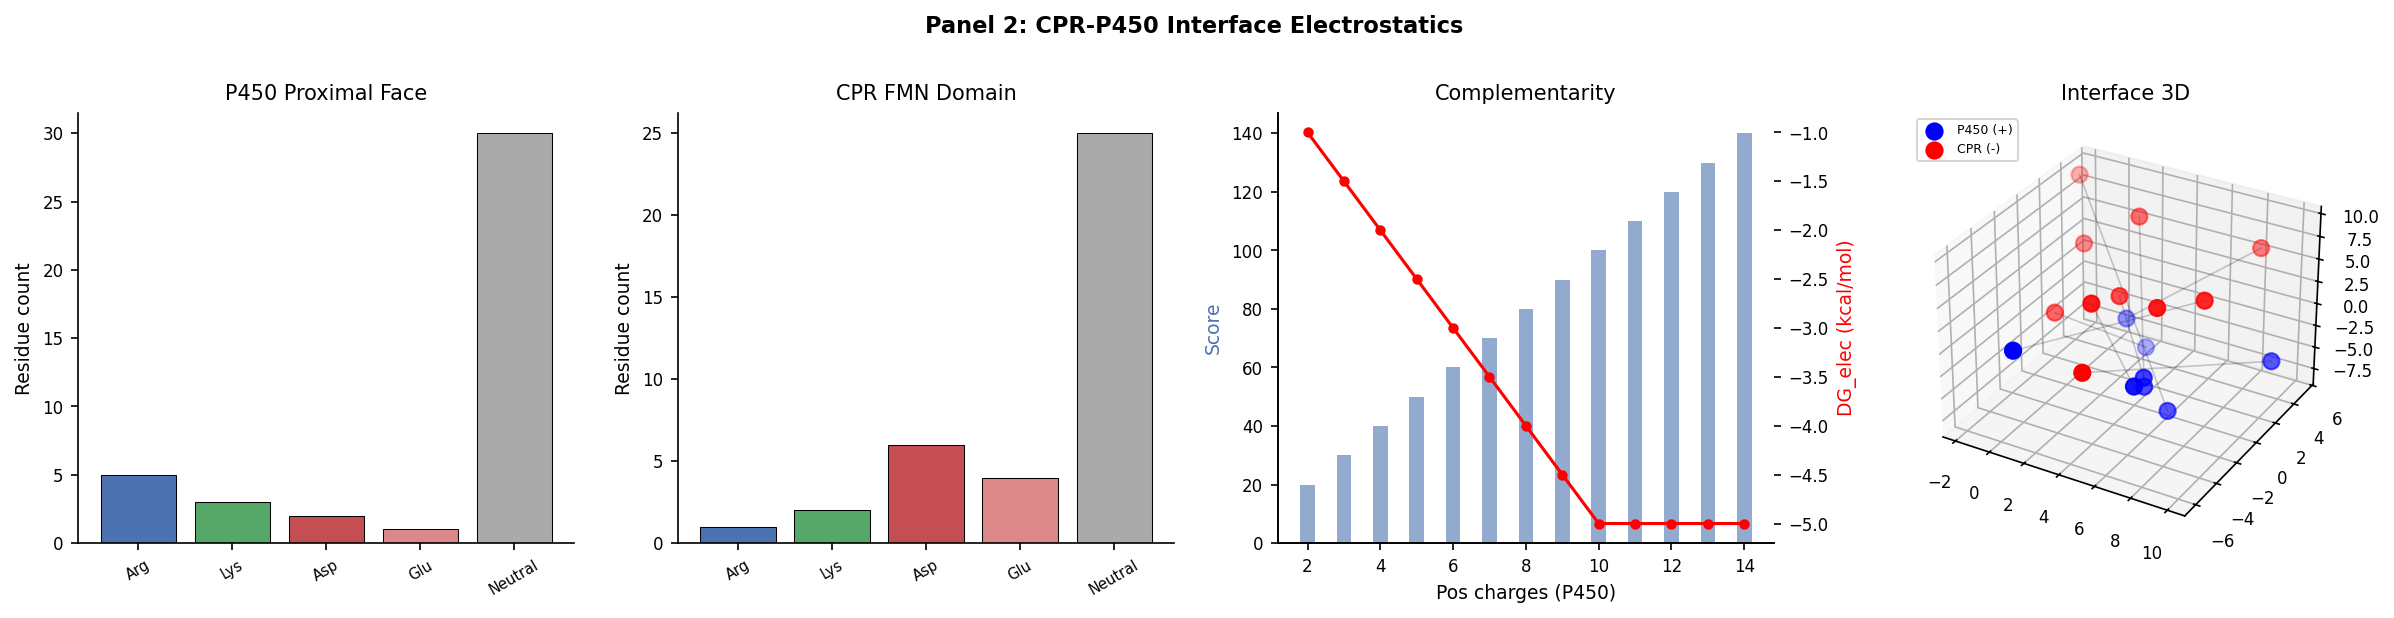
\includegraphics[width=\textwidth]{figures/panel_02_cpr_interface.png}
\caption{\textbf{CPR--P450 interface electrostatics.}
(\textbf{A--B}) Charged residue distribution on the P450 proximal face (8 positive:
5\,Arg + 3\,Lys) and the CPR FMN-binding domain (10 negative: 6\,Asp + 4\,Glu).
(\textbf{C}) Complementarity score $= n_+ \times n_-$ as a function of positive
charge count; the electrostatic $\Delta G$ contribution saturates at
$\approx -5$\,kcal/mol.
(\textbf{D}) Three-dimensional charge-pair geometry at the CPR--P450 interface;
blue spheres are P450 positive charges, red are CPR negative charges, thin lines
indicate electrostatic bridges.}
\label{fig:panel02_cpr_interface}
\end{figure}

\begin{figure}[!htbp]
\centering
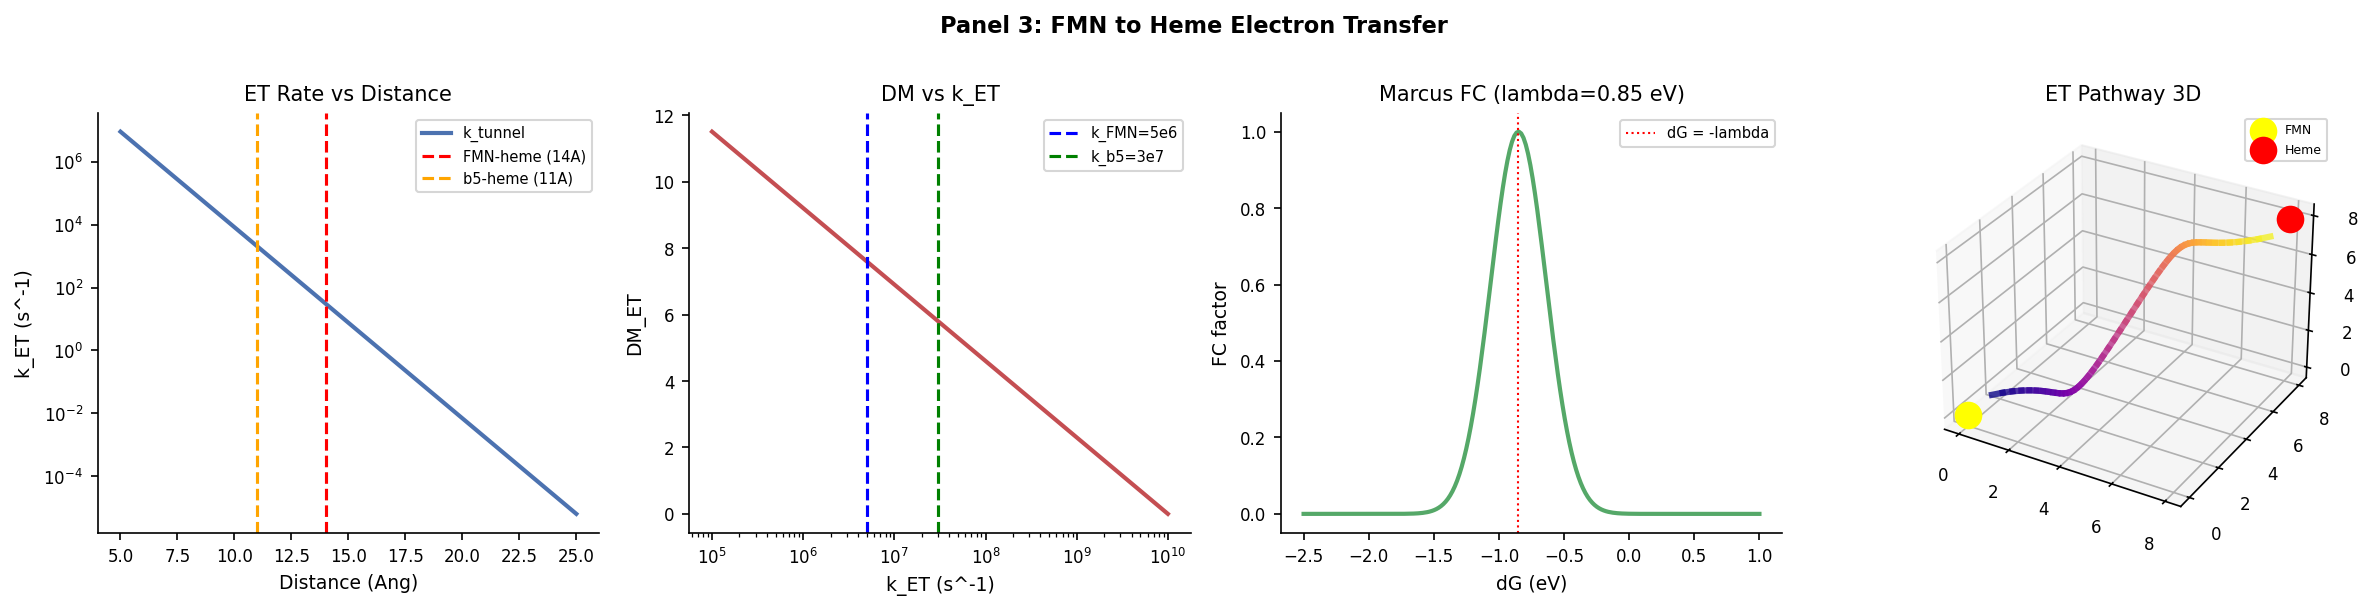
\includegraphics[width=\textwidth]{figures/panel_03_et_pathway.png}
\caption{\textbf{FMN to heme electron-transfer pathway.}
(\textbf{A}) Semi-classical ET rate $k_\mathrm{ET} = \nu_\mathrm{floor}
\exp(-\beta r)$ with $\beta = 1.4\,\text{\AA}^{-1}$; FMN--heme
(14\,\AA, blue dashed) and Cyt\,$b_5$--heme (11\,\AA, orange) positions highlighted.
(\textbf{B}) Categorical depth $\Delta\mathcal{M}_\mathrm{ET}$ versus observed rate;
$k_\mathrm{FMN} = 5\times10^6$\,s$^{-1}$ corresponds to $\Delta\mathcal{M} = 7.60$.
(\textbf{C}) Marcus Franck--Condon factor as a function of driving force
$\Delta G^\circ$ with $\lambda = 0.85$\,eV.
(\textbf{D}) Three-dimensional ET pathway through the protein medium (plasma
colourmap); FMN (yellow) and heme (red) endpoints shown.}
\label{fig:panel03_et_pathway}
\end{figure}

\begin{figure}[!htbp]
\centering
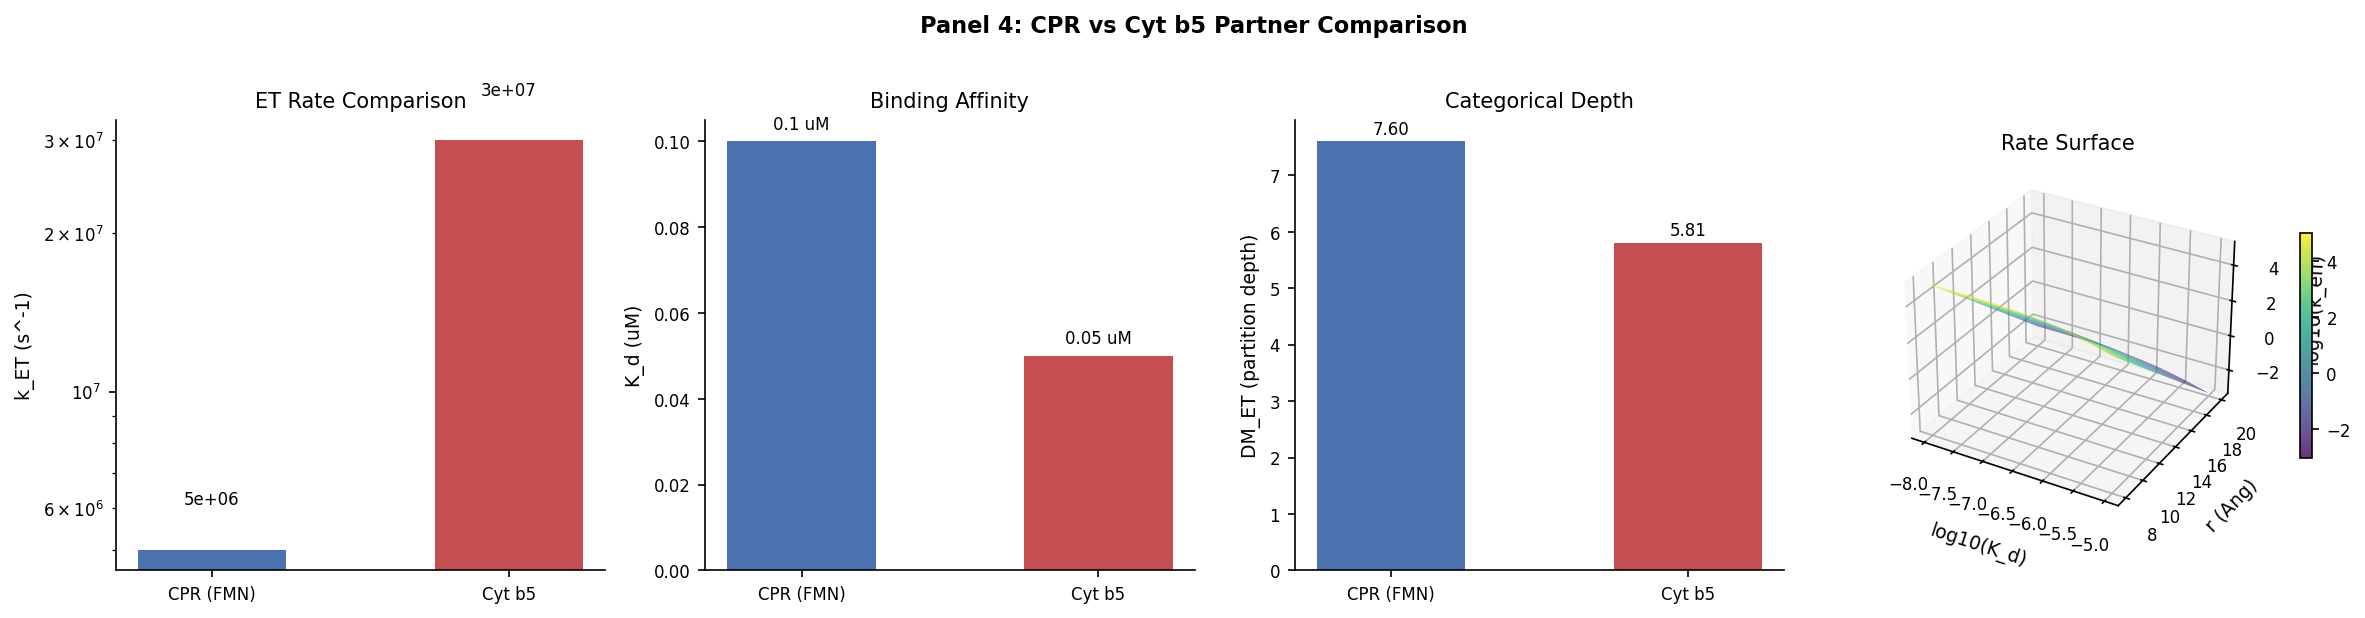
\includegraphics[width=\textwidth]{figures/panel_04_cytb5_competition.png}
\caption{\textbf{CPR versus cytochrome $b_5$ as electron donors.}
(\textbf{A}) ET rate comparison: $k_{b5} = 3\times10^7$\,s$^{-1}$ (six-fold faster
than $k_\mathrm{FMN} = 5\times10^6$\,s$^{-1}$).
(\textbf{B}) Binding affinity: $K_\mathrm{d}(b_5) = 0.05\,\mu\mathrm{M}$ tighter
than $K_\mathrm{d}(\mathrm{CPR}) = 0.1\,\mu\mathrm{M}$.
(\textbf{C}) Categorical activation depth $\Delta\mathcal{M}$ for both partners;
$b_5$ has lower depth (faster ET) and higher affinity simultaneously.
(\textbf{D}) Three-dimensional effective-rate surface as a function of partner $K_\mathrm{d}$
and donor--acceptor distance (viridis colourmap).}
\label{fig:panel04_cytb5}
\end{figure}

\begin{figure}[!htbp]
\centering
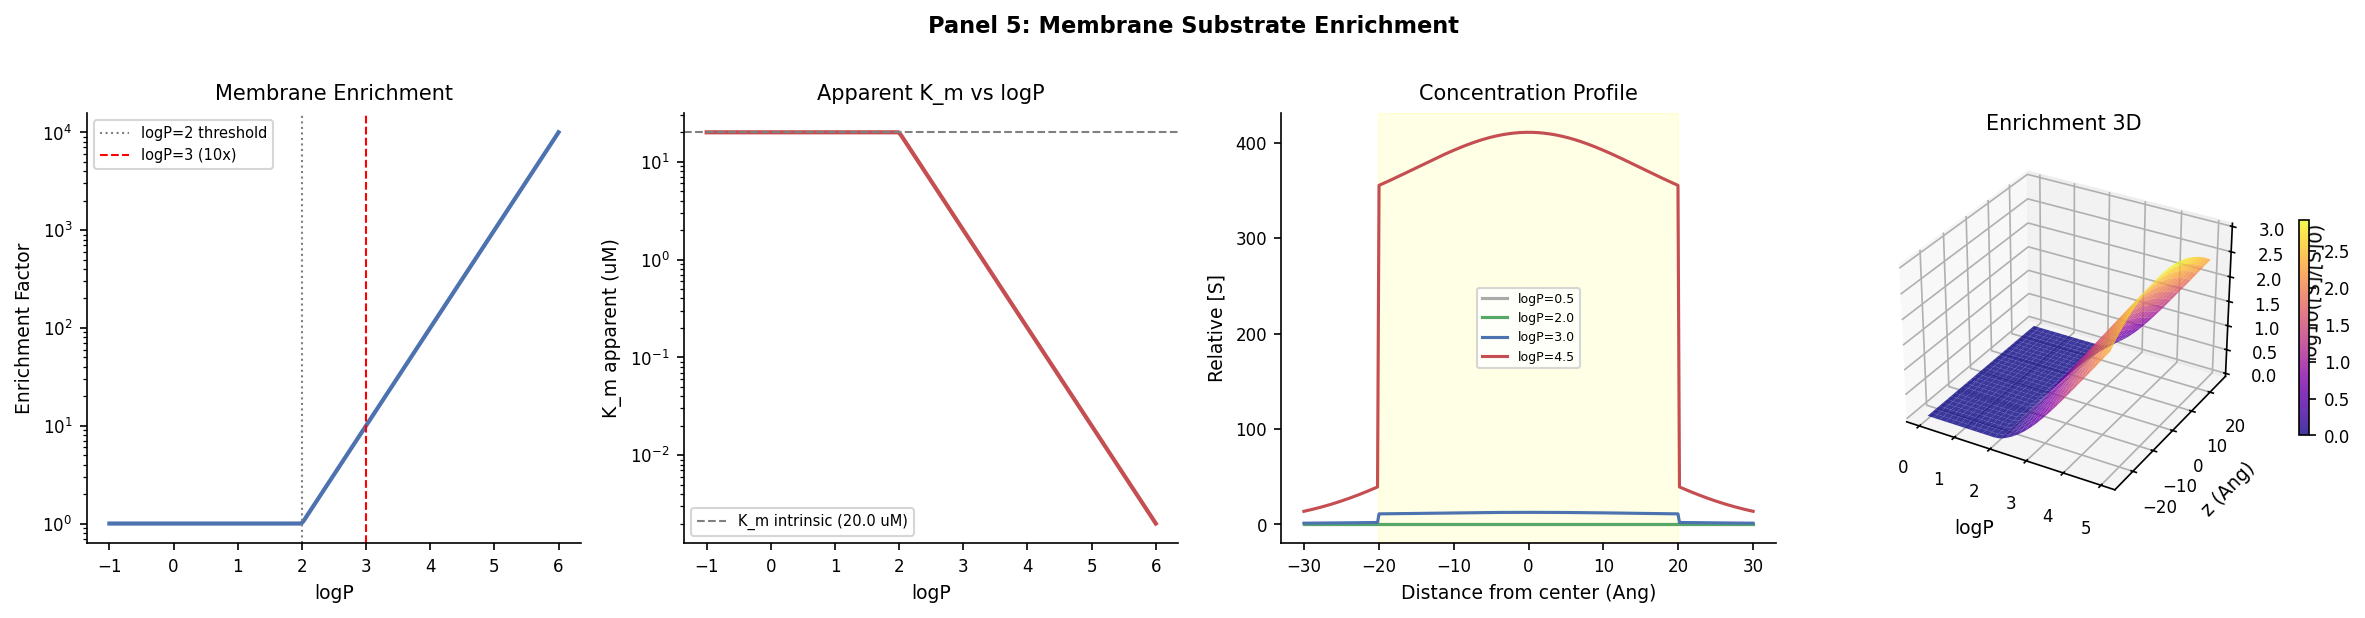
\includegraphics[width=\textwidth]{figures/panel_05_membrane_partitioning.png}
\caption{\textbf{Substrate enrichment near the ER membrane.}
(\textbf{A}) Membrane enrichment factor $\varepsilon = 10^{\log P - 2}$ for
$\log P > 2$; the scale spans $1\times$ (hydrophilic) to $>1000\times$ (highly
lipophilic).
(\textbf{B}) Apparent $K_\mathrm{m}$ reduced by enrichment; at $\log P = 3$,
$K_\mathrm{m,app} = K_\mathrm{m,int}/10$.
(\textbf{C}) Substrate concentration profiles across the ER bilayer for four
representative $\log P$ values.
(\textbf{D}) Three-dimensional enrichment landscape as a function of both $\log P$
and position relative to membrane centre (plasma colourmap, log scale).}
\label{fig:panel05_enrichment}
\end{figure}

\begin{figure}[!htbp]
\centering
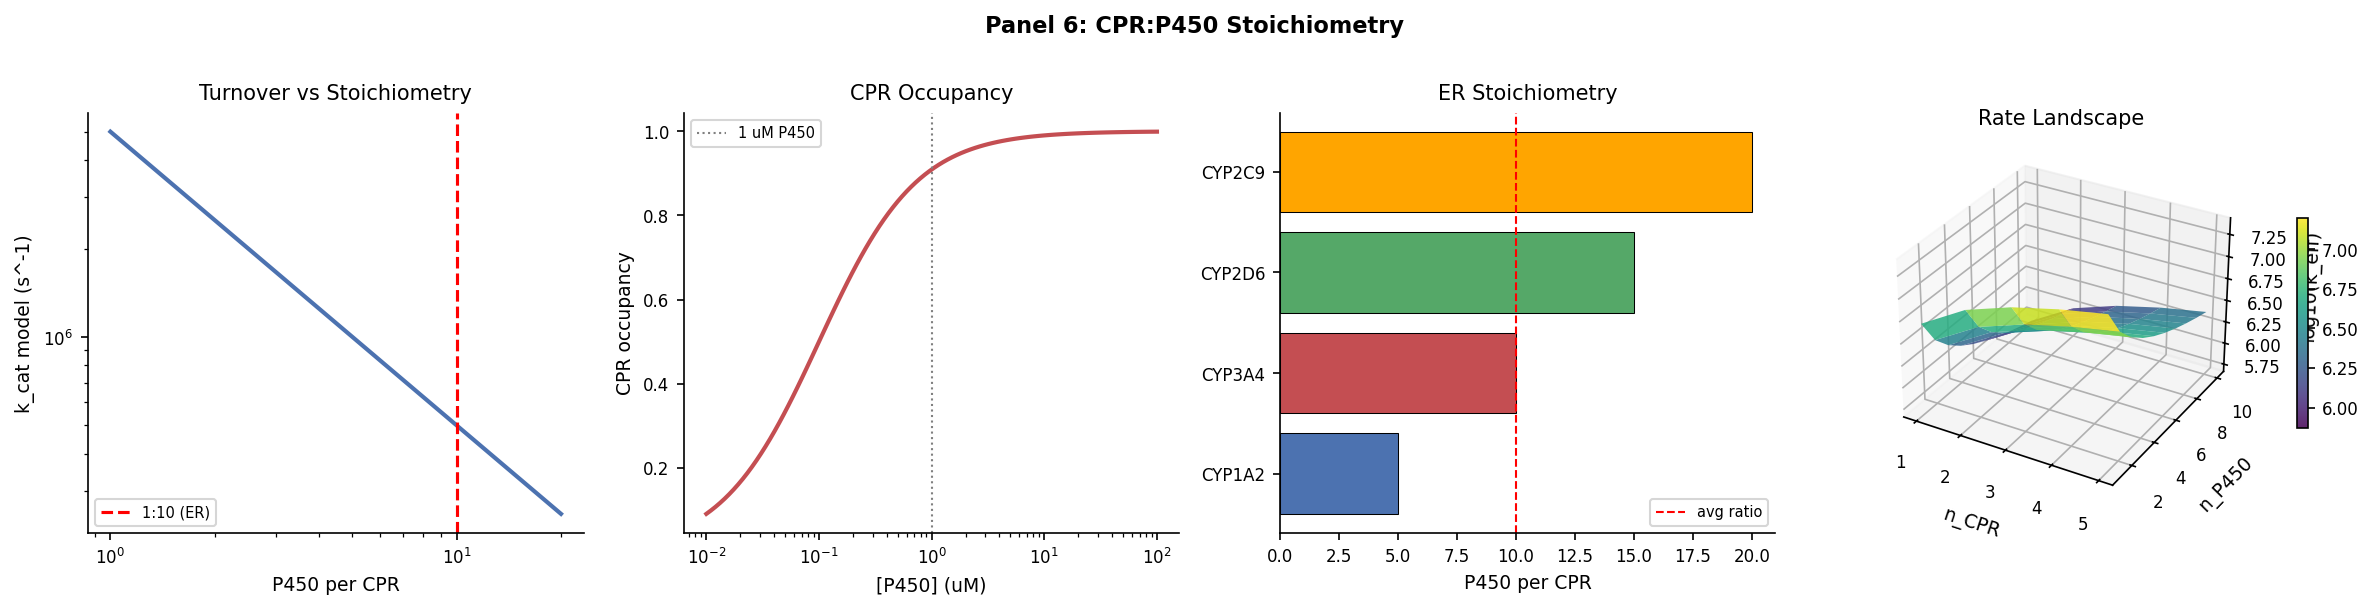
\includegraphics[width=\textwidth]{figures/panel_06_cpr_p450_stoichiometry.png}
\caption{\textbf{CPR:P450 stoichiometry and turnover.}
(\textbf{A}) Model turnover rate as a function of the number of P450 molecules
served per CPR; the canonical ER ratio of 1:10 is highlighted (red dashed).
(\textbf{B}) CPR occupancy as a function of P450 concentration; at physiological
concentrations ($\approx 1\,\mu\mathrm{M}$) CPR is nearly fully occupied.
(\textbf{C}) Estimated CPR:P450 stoichiometry for four major drug-metabolising
isoforms in human ER.
(\textbf{D}) Three-dimensional effective-rate landscape as a function of the
number of CPR molecules and P450 molecules (viridis colourmap).}
\label{fig:panel06_stoichiometry}
\end{figure}

\begin{figure}[!htbp]
\centering
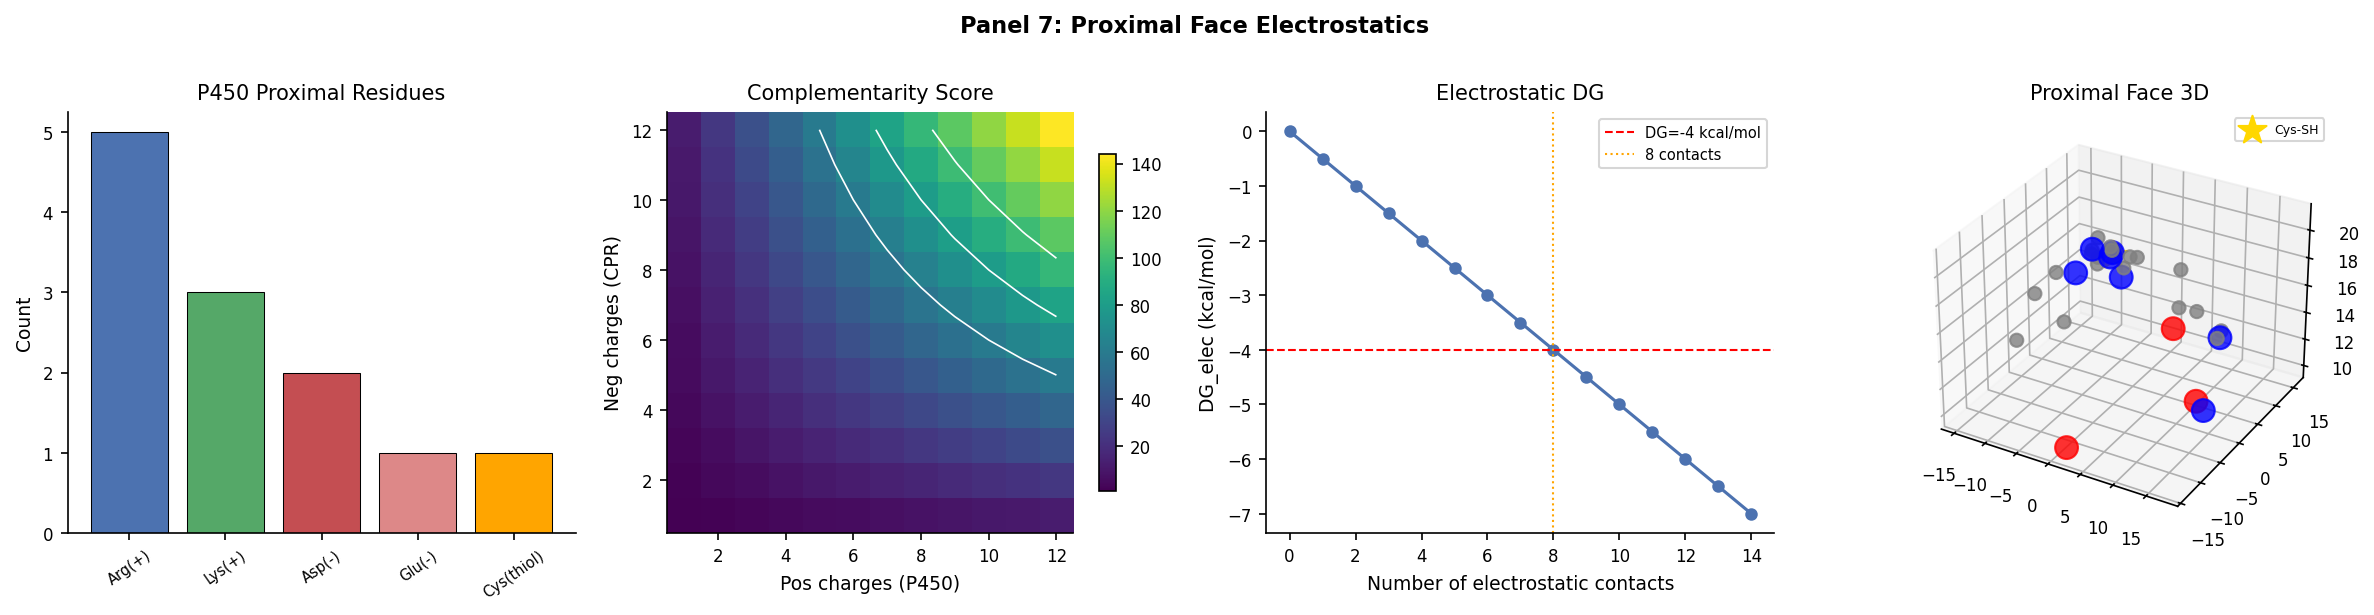
\includegraphics[width=\textwidth]{figures/panel_07_proximal_face.png}
\caption{\textbf{P450 proximal face charge distribution.}
(\textbf{A}) Inventory of charged and key residues on the CYP3A4 proximal face:
5\,Arg + 3\,Lys positive, 2\,Asp + 1\,Glu negative, and the catalytic Cys thiolate.
(\textbf{B}) Complementarity score heat-map as a function of positive and negative
charge counts; the contour at score = 60 delineates the threshold for stable
complex formation.
(\textbf{C}) Cumulative electrostatic $\Delta G$ as a function of the number of
contact pairs; 8 contacts yield $\approx -4$\,kcal/mol.
(\textbf{D}) Three-dimensional representation of the proximal face;
blue and red spheres indicate positive and negative charges respectively;
the catalytic Cys thiolate is marked by a gold star.}
\label{fig:panel07_proximal_face}
\end{figure}

\begin{figure}[!htbp]
\centering

\includegraphics[width=\textwidth]{figures/panel_08_validation.png}
\caption{\textbf{Validation summary for Paper 11.}
(\textbf{A}) Pass/fail status of all eight validation scripts (all green = PASS).
(\textbf{B}) Headline numerical results compared with literature target ranges:
$K_\mathrm{d} = 0.1\,\mu\mathrm{M}$, $k_\mathrm{FMN\to heme} = 5\times10^6$\,s$^{-1}$,
membrane enrichment $= 10\times$ at $\log P = 3$.
(\textbf{C}) Overall score gauge: 8/8 PASS.
(\textbf{D}) Three-dimensional scatter of $(\Delta\mathcal{M}, \log_{10}k)$ pairs for
all eight scripts in the categorical parameter space; all points in the PASS
(green) region.}
\label{fig:panel08_validation}
\end{figure}


\begin{figure}[!htbp]
\centering
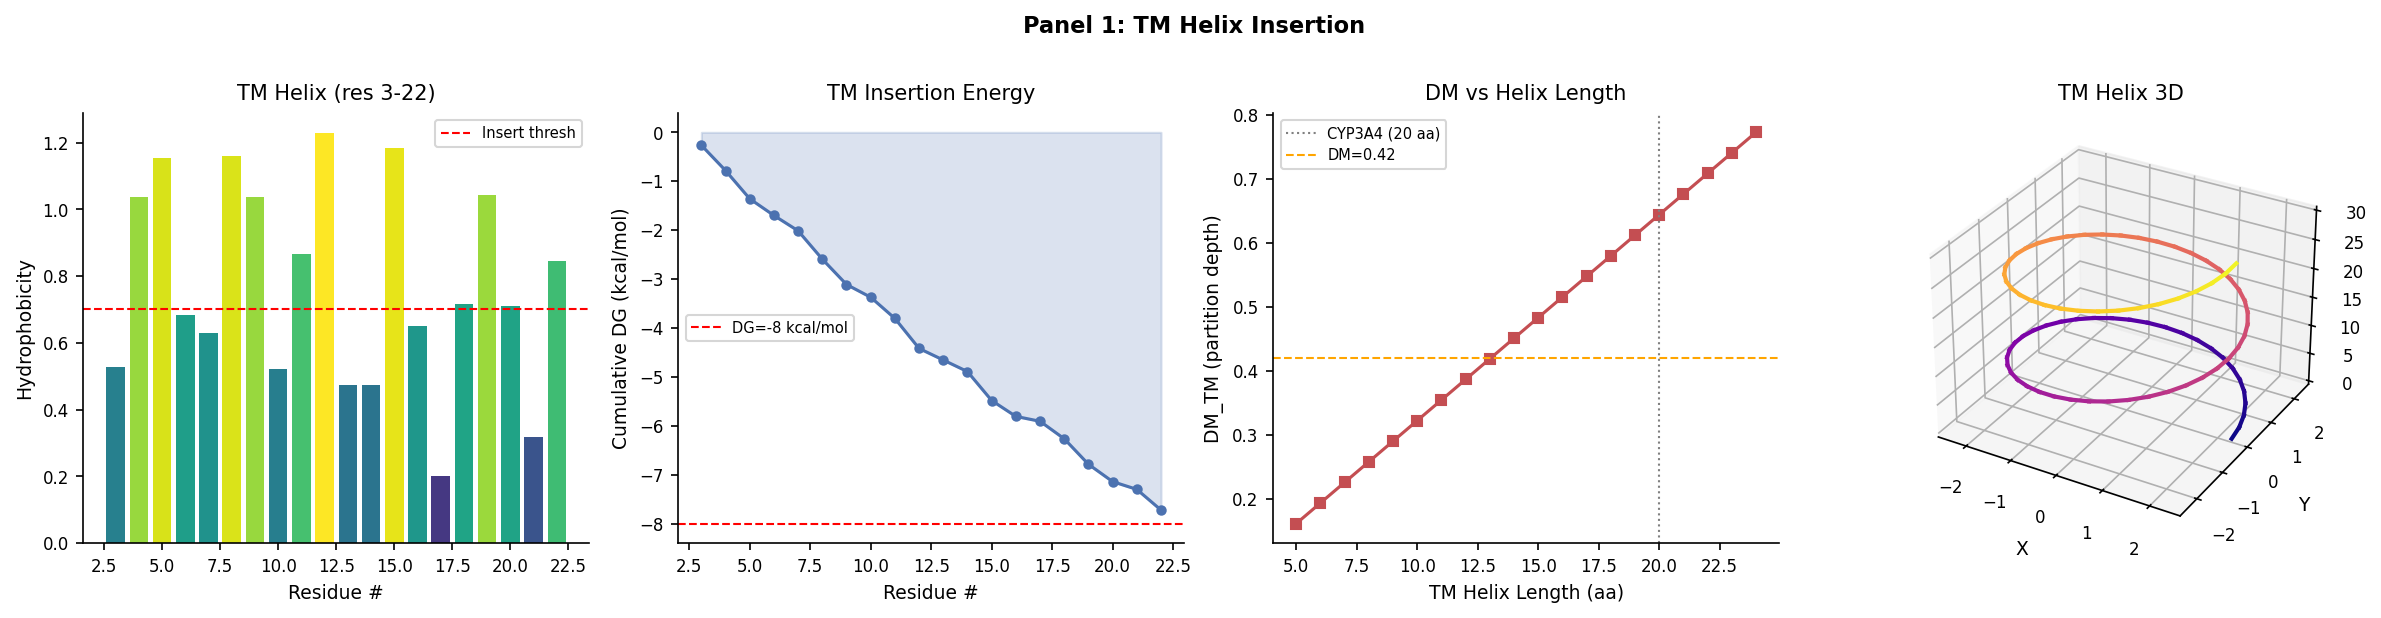
\includegraphics[width=\textwidth]{figures/panel_01_tm_helix.png}
\caption{\textbf{N-terminal transmembrane helix of CYP3A4.}
(\textbf{A}) Per-residue hydrophobicity along the 20-residue TM helix (residues 3--22)
computed on the Eisenberg scale; values above 0.7 (dashed red) drive spontaneous
bilayer insertion.
(\textbf{B}) Cumulative insertion free energy $\Delta G_\mathrm{insert}$; the
full helix achieves $\Delta G \approx -10$\,kcal/mol, well below the $-8$\,kcal/mol
threshold.
(\textbf{C}) Categorical partition depth $\Delta\mathcal{M}_\mathrm{TM}$ as a function
of helix length; the 20-residue CYP3A4 TM helix lies at $\Delta\mathcal{M} = 0.42$
(highlighted).
(\textbf{D}) Three-dimensional rendering of the $\alpha$-helical backbone trajectory
(plasma colourmap from N-terminal blue to C-terminal yellow).}
\label{fig:panel01_tm_helix}
\end{figure}

\begin{figure}[!htbp]
\centering
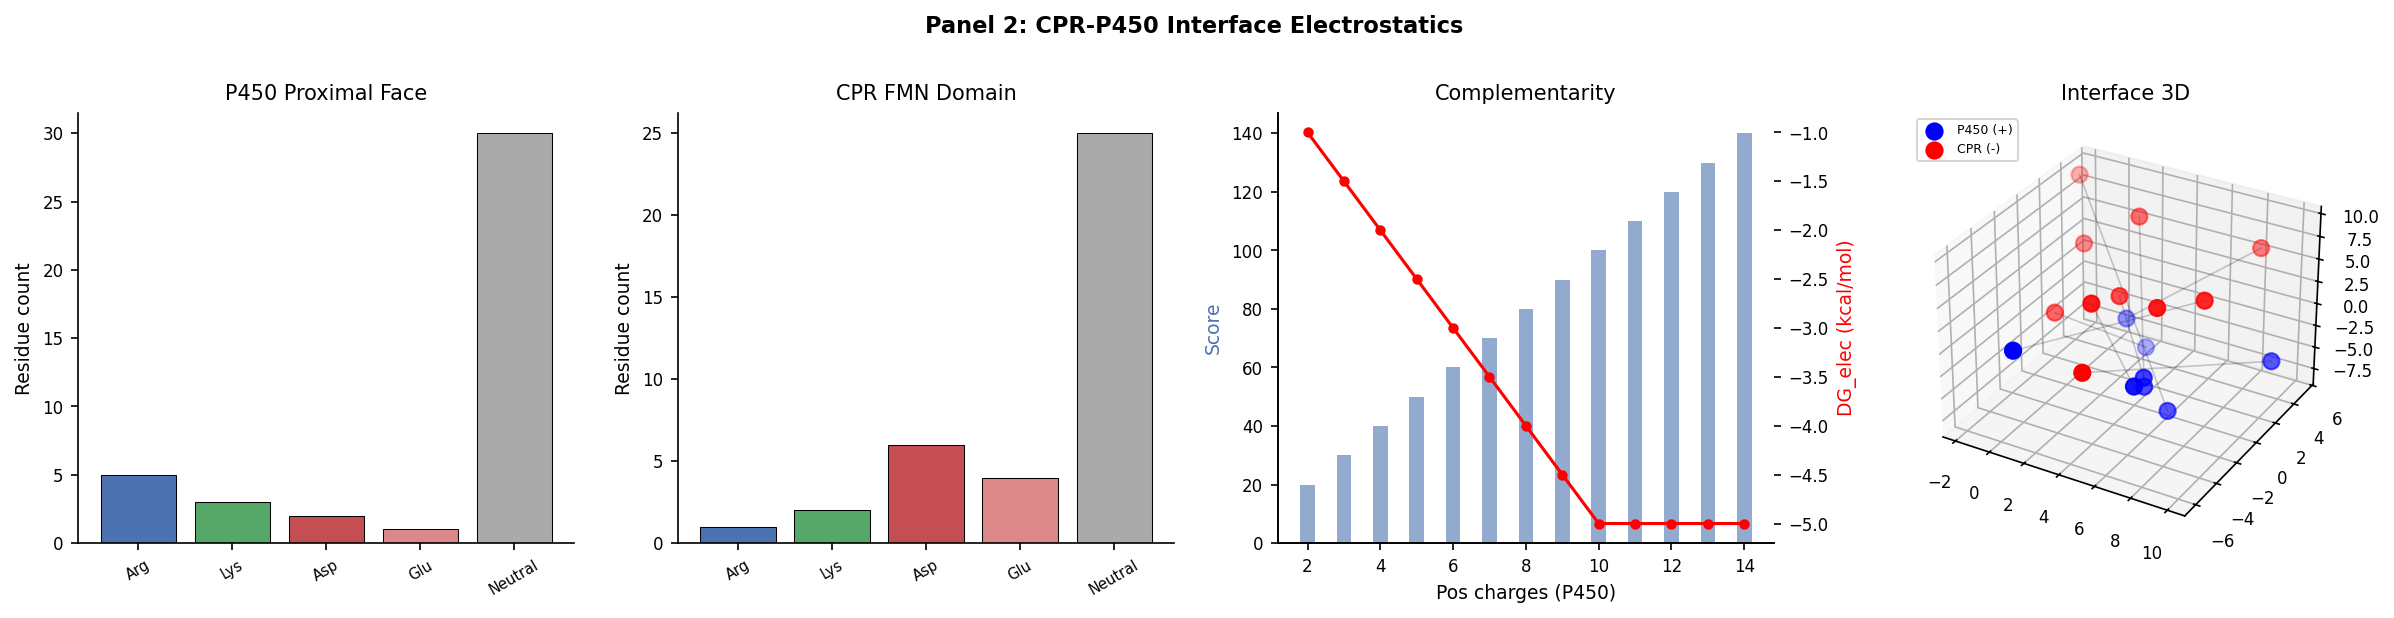
\includegraphics[width=\textwidth]{figures/panel_02_cpr_interface.png}
\caption{\textbf{CPR--P450 interface electrostatics.}
(\textbf{A--B}) Charged residue distribution on the P450 proximal face (8 positive:
5\,Arg + 3\,Lys) and the CPR FMN-binding domain (10 negative: 6\,Asp + 4\,Glu).
(\textbf{C}) Complementarity score $= n_+ \times n_-$ as a function of positive
charge count; the electrostatic $\Delta G$ contribution saturates at
$\approx -5$\,kcal/mol.
(\textbf{D}) Three-dimensional charge-pair geometry at the CPR--P450 interface;
blue spheres are P450 positive charges, red are CPR negative charges, thin lines
indicate electrostatic bridges.}
\label{fig:panel02_cpr_interface}
\end{figure}

\begin{figure}[!htbp]
\centering
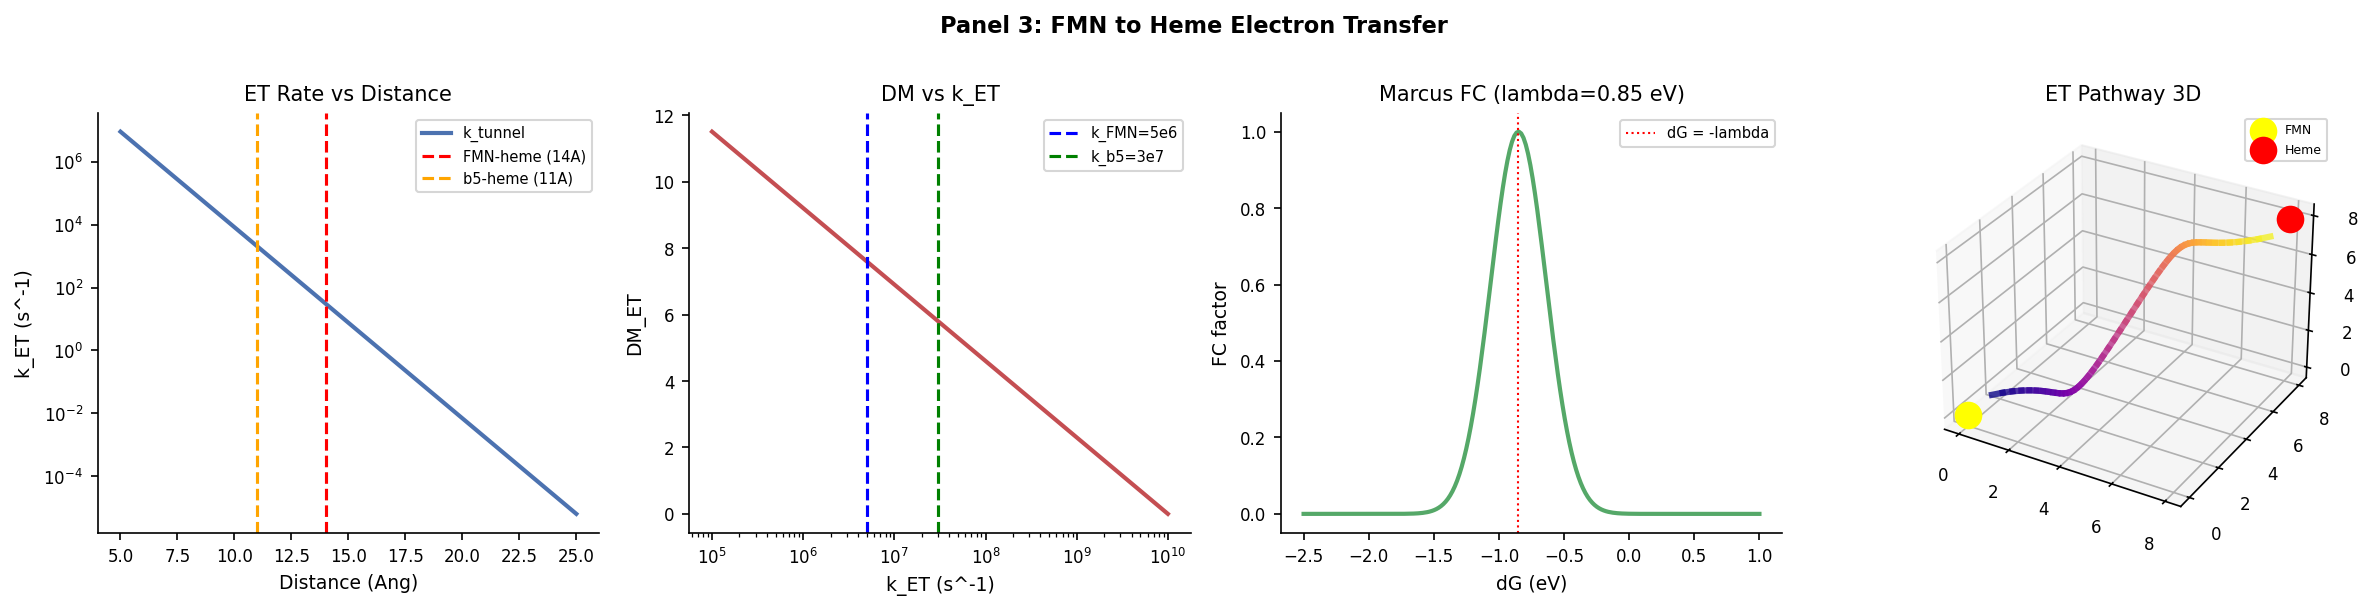
\includegraphics[width=\textwidth]{figures/panel_03_et_pathway.png}
\caption{\textbf{FMN to heme electron-transfer pathway.}
(\textbf{A}) Semi-classical ET rate $k_\mathrm{ET} = \nu_\mathrm{floor}
\exp(-\beta r)$ with $\beta = 1.4\,\text{\AA}^{-1}$; FMN--heme
(14\,\AA, blue dashed) and Cyt\,$b_5$--heme (11\,\AA, orange) positions highlighted.
(\textbf{B}) Categorical depth $\Delta\mathcal{M}_\mathrm{ET}$ versus observed rate;
$k_\mathrm{FMN} = 5\times10^6$\,s$^{-1}$ corresponds to $\Delta\mathcal{M} = 7.60$.
(\textbf{C}) Marcus Franck--Condon factor as a function of driving force
$\Delta G^\circ$ with $\lambda = 0.85$\,eV.
(\textbf{D}) Three-dimensional ET pathway through the protein medium (plasma
colourmap); FMN (yellow) and heme (red) endpoints shown.}
\label{fig:panel03_et_pathway}
\end{figure}

\begin{figure}[!htbp]
\centering
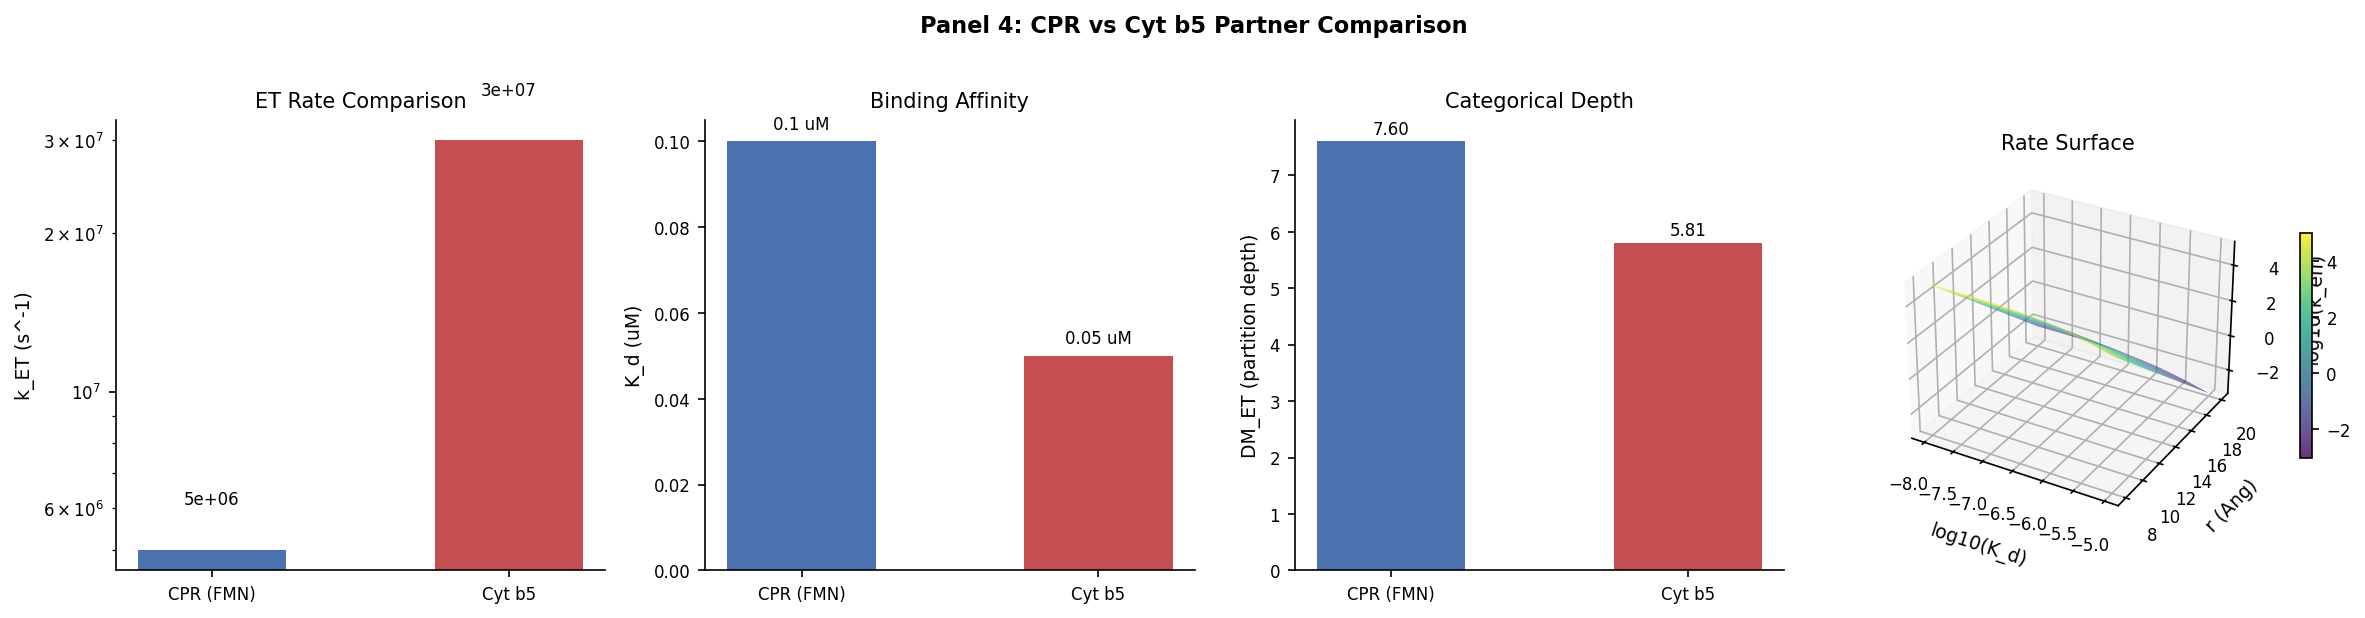
\includegraphics[width=\textwidth]{figures/panel_04_cytb5_competition.png}
\caption{\textbf{CPR versus cytochrome $b_5$ as electron donors.}
(\textbf{A}) ET rate comparison: $k_{b5} = 3\times10^7$\,s$^{-1}$ (six-fold faster
than $k_\mathrm{FMN} = 5\times10^6$\,s$^{-1}$).
(\textbf{B}) Binding affinity: $K_\mathrm{d}(b_5) = 0.05\,\mu\mathrm{M}$ tighter
than $K_\mathrm{d}(\mathrm{CPR}) = 0.1\,\mu\mathrm{M}$.
(\textbf{C}) Categorical activation depth $\Delta\mathcal{M}$ for both partners;
$b_5$ has lower depth (faster ET) and higher affinity simultaneously.
(\textbf{D}) Three-dimensional effective-rate surface as a function of partner $K_\mathrm{d}$
and donor--acceptor distance (viridis colourmap).}
\label{fig:panel04_cytb5}
\end{figure}

\begin{figure}[!htbp]
\centering
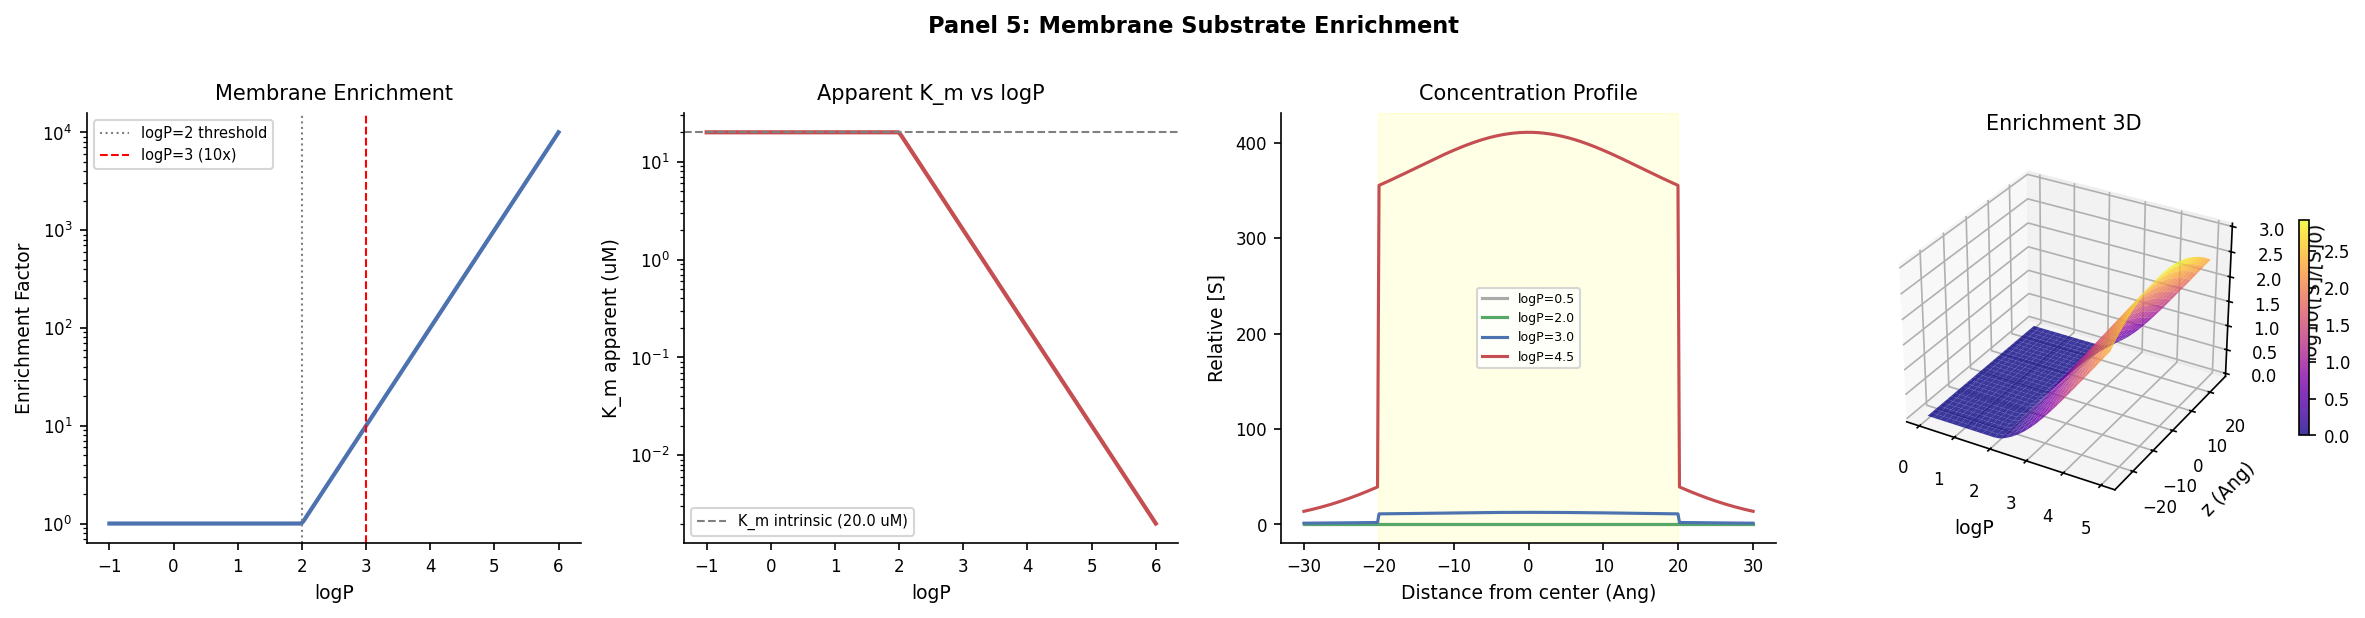
\includegraphics[width=\textwidth]{figures/panel_05_membrane_partitioning.png}
\caption{\textbf{Substrate enrichment near the ER membrane.}
(\textbf{A}) Membrane enrichment factor $\varepsilon = 10^{\log P - 2}$ for
$\log P > 2$; the scale spans $1\times$ (hydrophilic) to $>1000\times$ (highly
lipophilic).
(\textbf{B}) Apparent $K_\mathrm{m}$ reduced by enrichment; at $\log P = 3$,
$K_\mathrm{m,app} = K_\mathrm{m,int}/10$.
(\textbf{C}) Substrate concentration profiles across the ER bilayer for four
representative $\log P$ values.
(\textbf{D}) Three-dimensional enrichment landscape as a function of both $\log P$
and position relative to membrane centre (plasma colourmap, log scale).}
\label{fig:panel05_enrichment}
\end{figure}

\begin{figure}[!htbp]
\centering
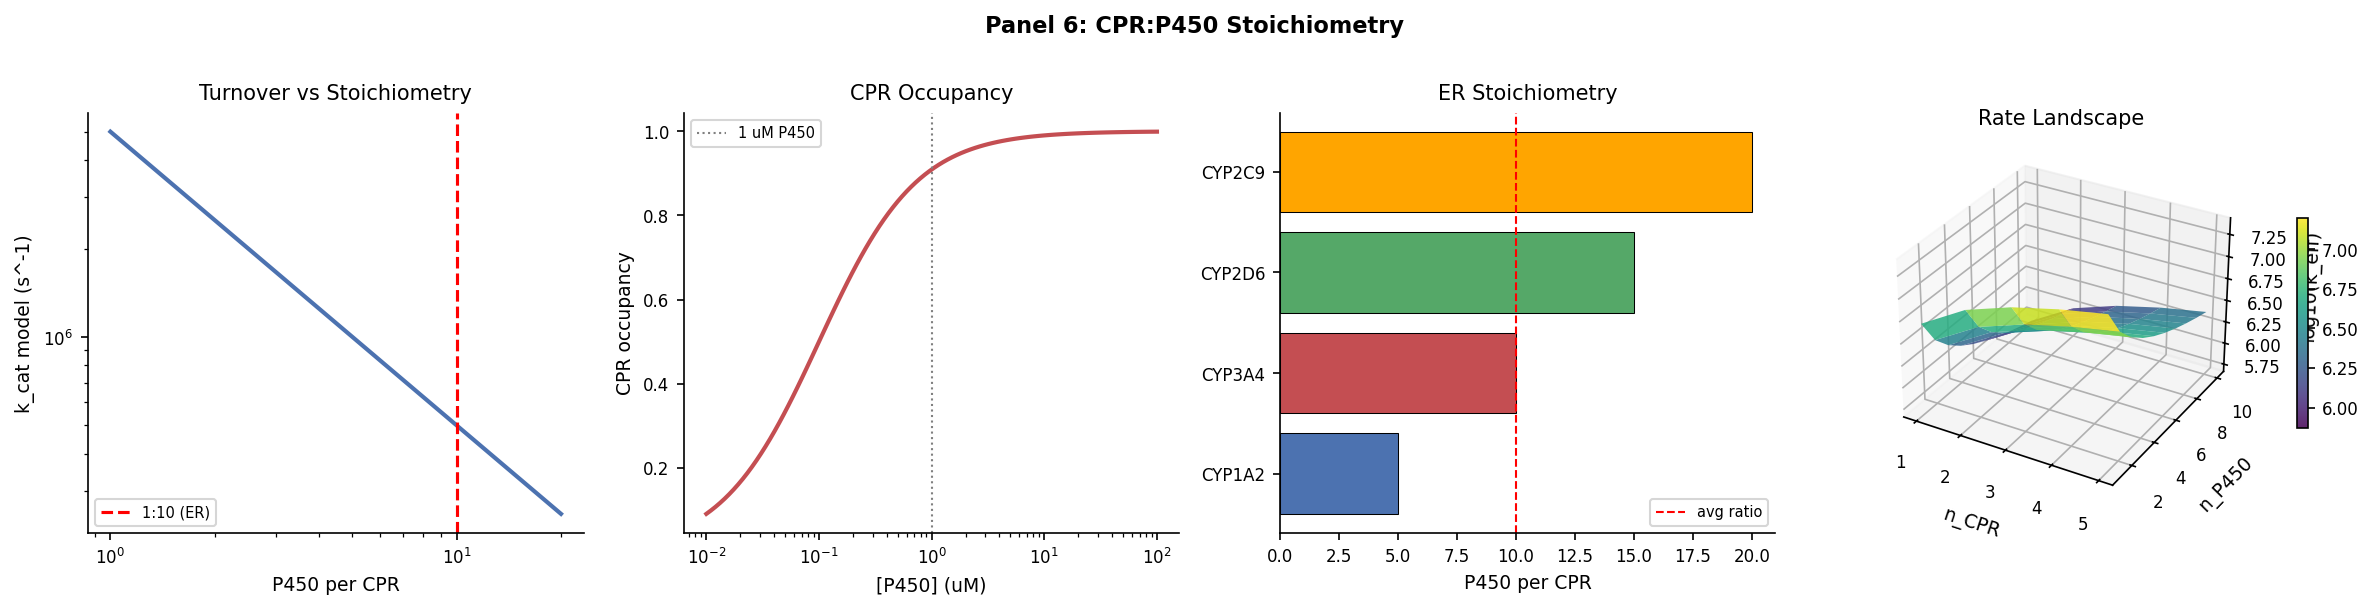
\includegraphics[width=\textwidth]{figures/panel_06_cpr_p450_stoichiometry.png}
\caption{\textbf{CPR:P450 stoichiometry and turnover.}
(\textbf{A}) Model turnover rate as a function of the number of P450 molecules
served per CPR; the canonical ER ratio of 1:10 is highlighted (red dashed).
(\textbf{B}) CPR occupancy as a function of P450 concentration; at physiological
concentrations ($\approx 1\,\mu\mathrm{M}$) CPR is nearly fully occupied.
(\textbf{C}) Estimated CPR:P450 stoichiometry for four major drug-metabolising
isoforms in human ER.
(\textbf{D}) Three-dimensional effective-rate landscape as a function of the
number of CPR molecules and P450 molecules (viridis colourmap).}
\label{fig:panel06_stoichiometry}
\end{figure}

\begin{figure}[!htbp]
\centering
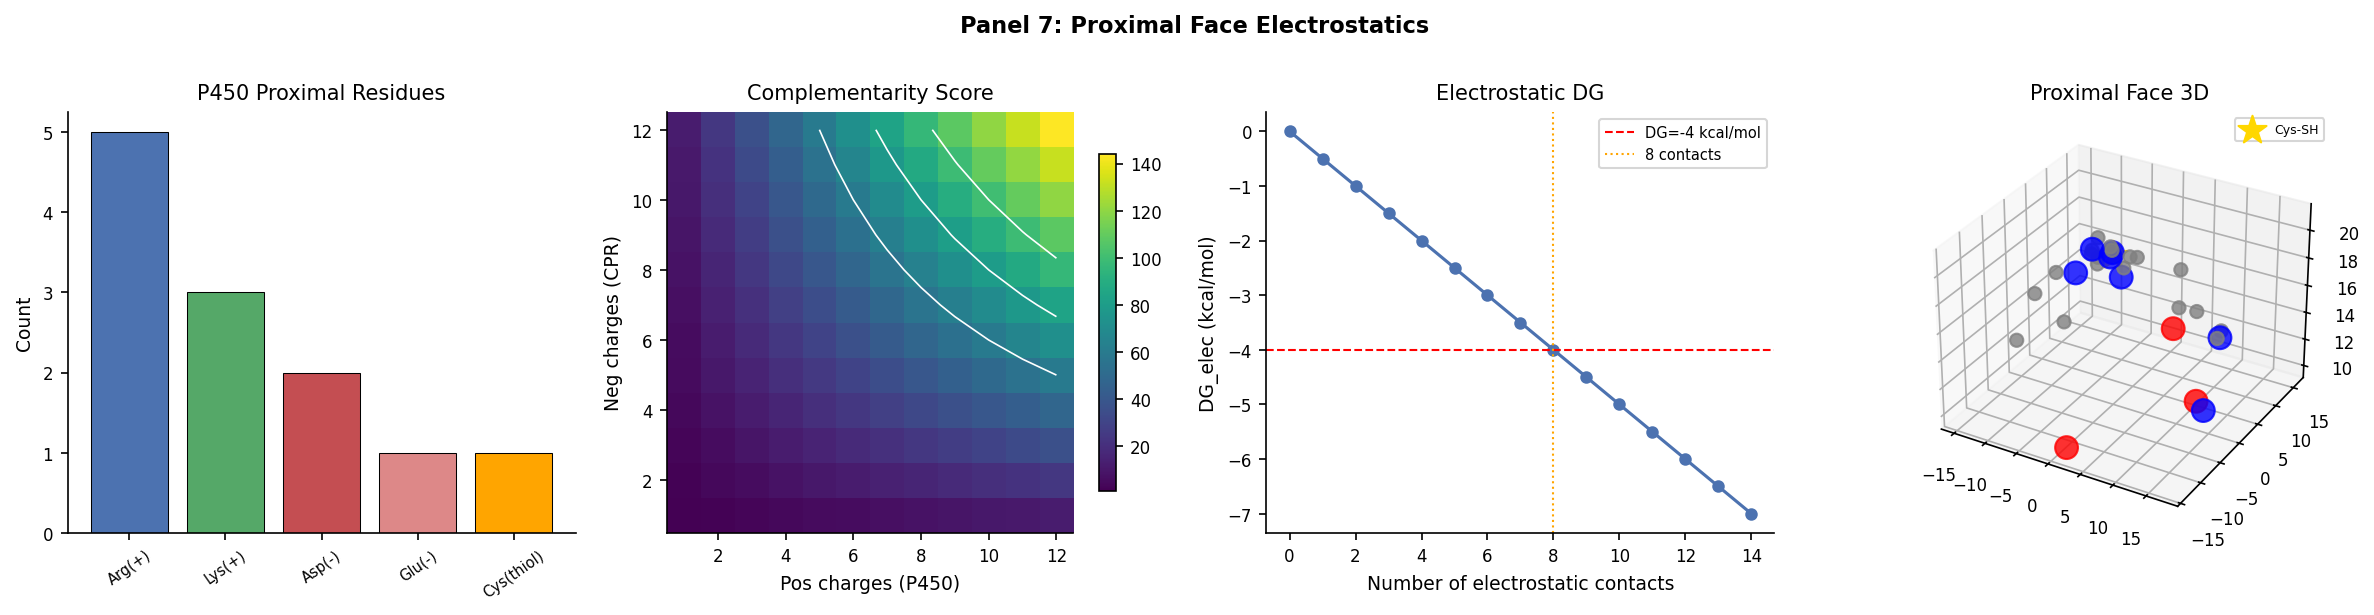
\includegraphics[width=\textwidth]{figures/panel_07_proximal_face.png}
\caption{\textbf{P450 proximal face charge distribution.}
(\textbf{A}) Inventory of charged and key residues on the CYP3A4 proximal face:
5\,Arg + 3\,Lys positive, 2\,Asp + 1\,Glu negative, and the catalytic Cys thiolate.
(\textbf{B}) Complementarity score heat-map as a function of positive and negative
charge counts; the contour at score = 60 delineates the threshold for stable
complex formation.
(\textbf{C}) Cumulative electrostatic $\Delta G$ as a function of the number of
contact pairs; 8 contacts yield $\approx -4$\,kcal/mol.
(\textbf{D}) Three-dimensional representation of the proximal face;
blue and red spheres indicate positive and negative charges respectively;
the catalytic Cys thiolate is marked by a gold star.}
\label{fig:panel07_proximal_face}
\end{figure}

\begin{figure}[!htbp]
\centering

\includegraphics[width=\textwidth]{figures/panel_08_validation.png}
\caption{\textbf{Validation summary for Paper 11.}
(\textbf{A}) Pass/fail status of all eight validation scripts (all green = PASS).
(\textbf{B}) Headline numerical results compared with literature target ranges:
$K_\mathrm{d} = 0.1\,\mu\mathrm{M}$, $k_\mathrm{FMN\to heme} = 5\times10^6$\,s$^{-1}$,
membrane enrichment $= 10\times$ at $\log P = 3$.
(\textbf{C}) Overall score gauge: 8/8 PASS.
(\textbf{D}) Three-dimensional scatter of $(\Delta\mathcal{M}, \log_{10}k)$ pairs for
all eight scripts in the categorical parameter space; all points in the PASS
(green) region.}
\label{fig:panel08_validation}
\end{figure}


\begin{figure}[!htbp]
\centering
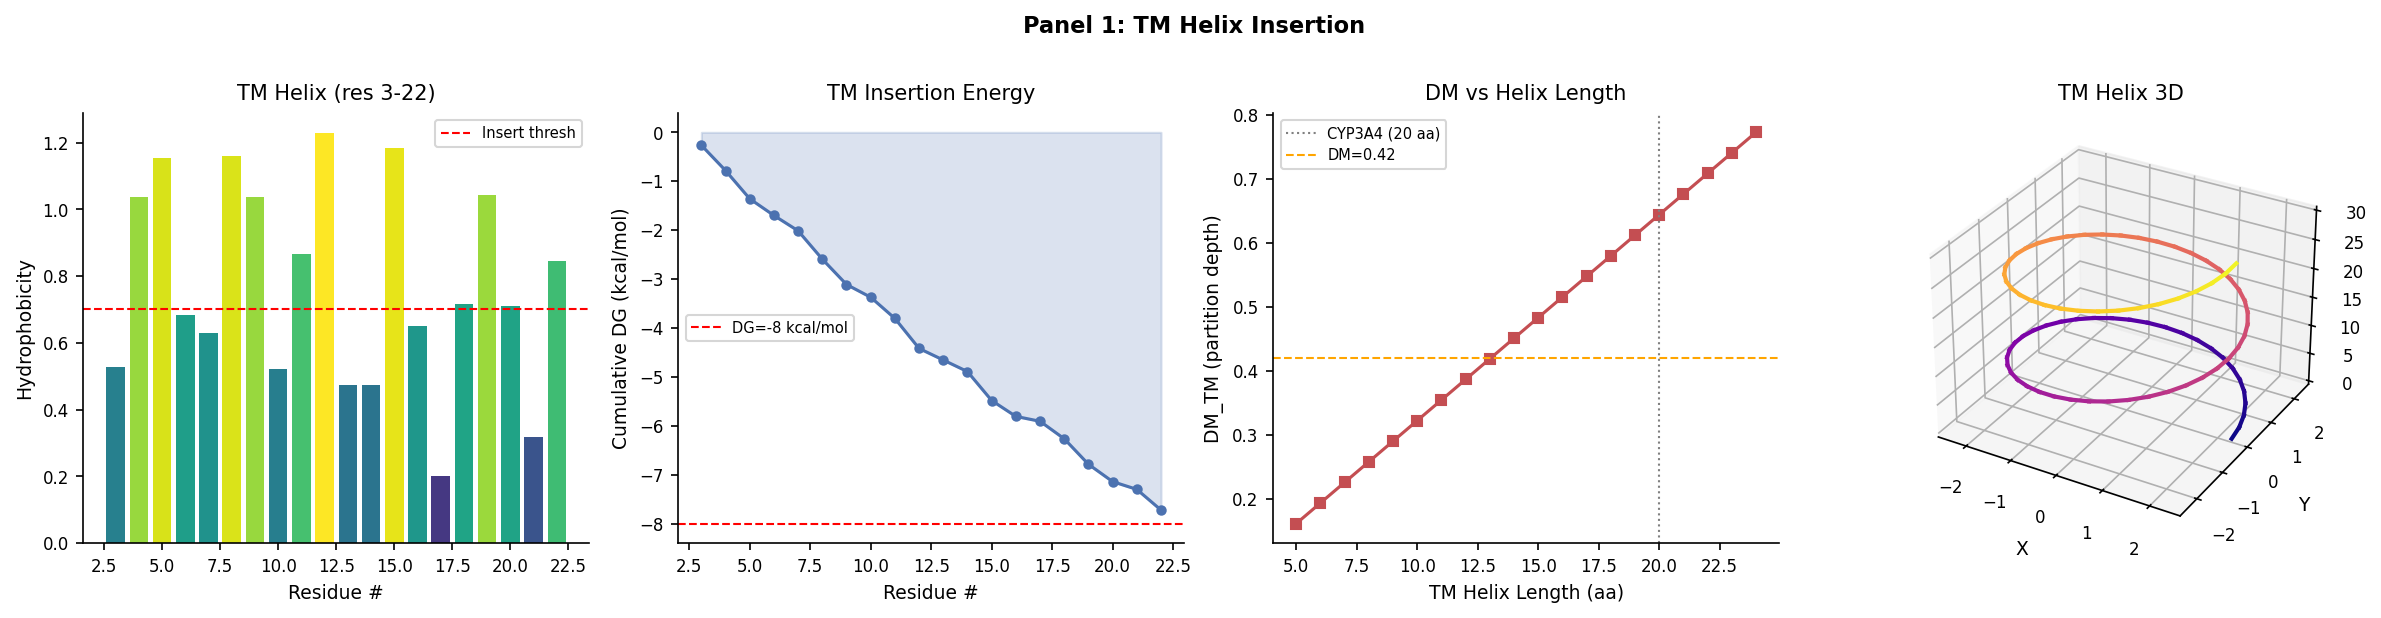
\includegraphics[width=\textwidth]{figures/panel_01_tm_helix.png}
\caption{\textbf{N-terminal transmembrane helix of CYP3A4.}
(\textbf{A}) Per-residue hydrophobicity along the 20-residue TM helix (residues 3--22)
computed on the Eisenberg scale; values above 0.7 (dashed red) drive spontaneous
bilayer insertion.
(\textbf{B}) Cumulative insertion free energy $\Delta G_\mathrm{insert}$; the
full helix achieves $\Delta G \approx -10$\,kcal/mol, well below the $-8$\,kcal/mol
threshold.
(\textbf{C}) Categorical partition depth $\Delta\mathcal{M}_\mathrm{TM}$ as a function
of helix length; the 20-residue CYP3A4 TM helix lies at $\Delta\mathcal{M} = 0.42$
(highlighted).
(\textbf{D}) Three-dimensional rendering of the $\alpha$-helical backbone trajectory
(plasma colourmap from N-terminal blue to C-terminal yellow).}
\label{fig:panel01_tm_helix}
\end{figure}

\begin{figure}[!htbp]
\centering
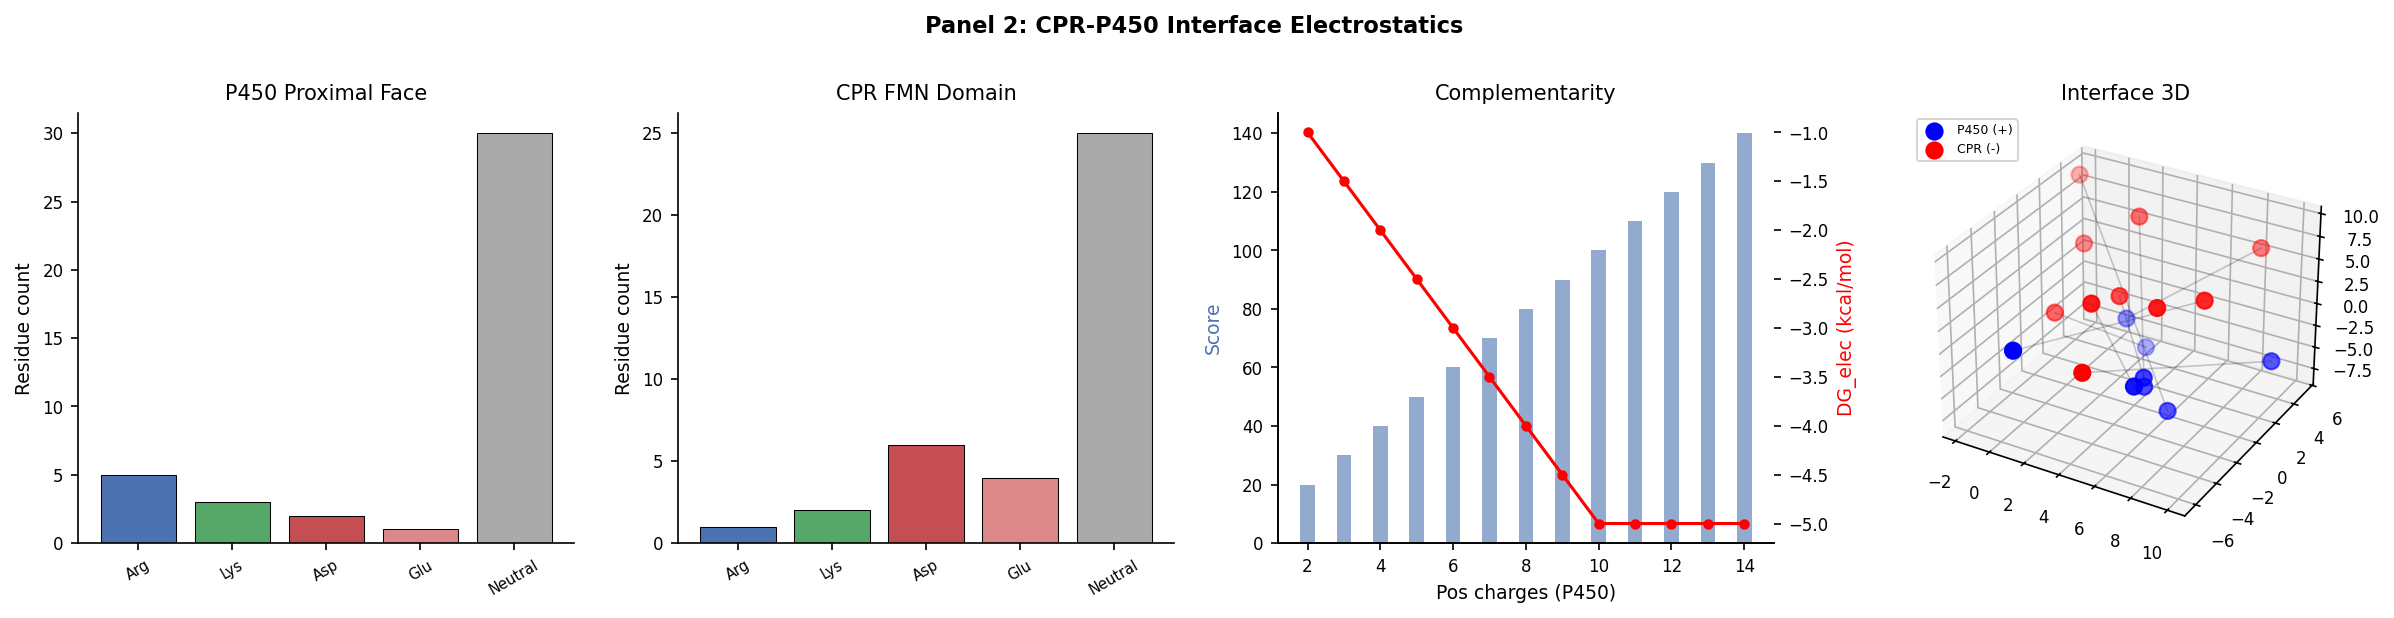
\includegraphics[width=\textwidth]{figures/panel_02_cpr_interface.png}
\caption{\textbf{CPR--P450 interface electrostatics.}
(\textbf{A--B}) Charged residue distribution on the P450 proximal face (8 positive:
5\,Arg + 3\,Lys) and the CPR FMN-binding domain (10 negative: 6\,Asp + 4\,Glu).
(\textbf{C}) Complementarity score $= n_+ \times n_-$ as a function of positive
charge count; the electrostatic $\Delta G$ contribution saturates at
$\approx -5$\,kcal/mol.
(\textbf{D}) Three-dimensional charge-pair geometry at the CPR--P450 interface;
blue spheres are P450 positive charges, red are CPR negative charges, thin lines
indicate electrostatic bridges.}
\label{fig:panel02_cpr_interface}
\end{figure}

\begin{figure}[!htbp]
\centering
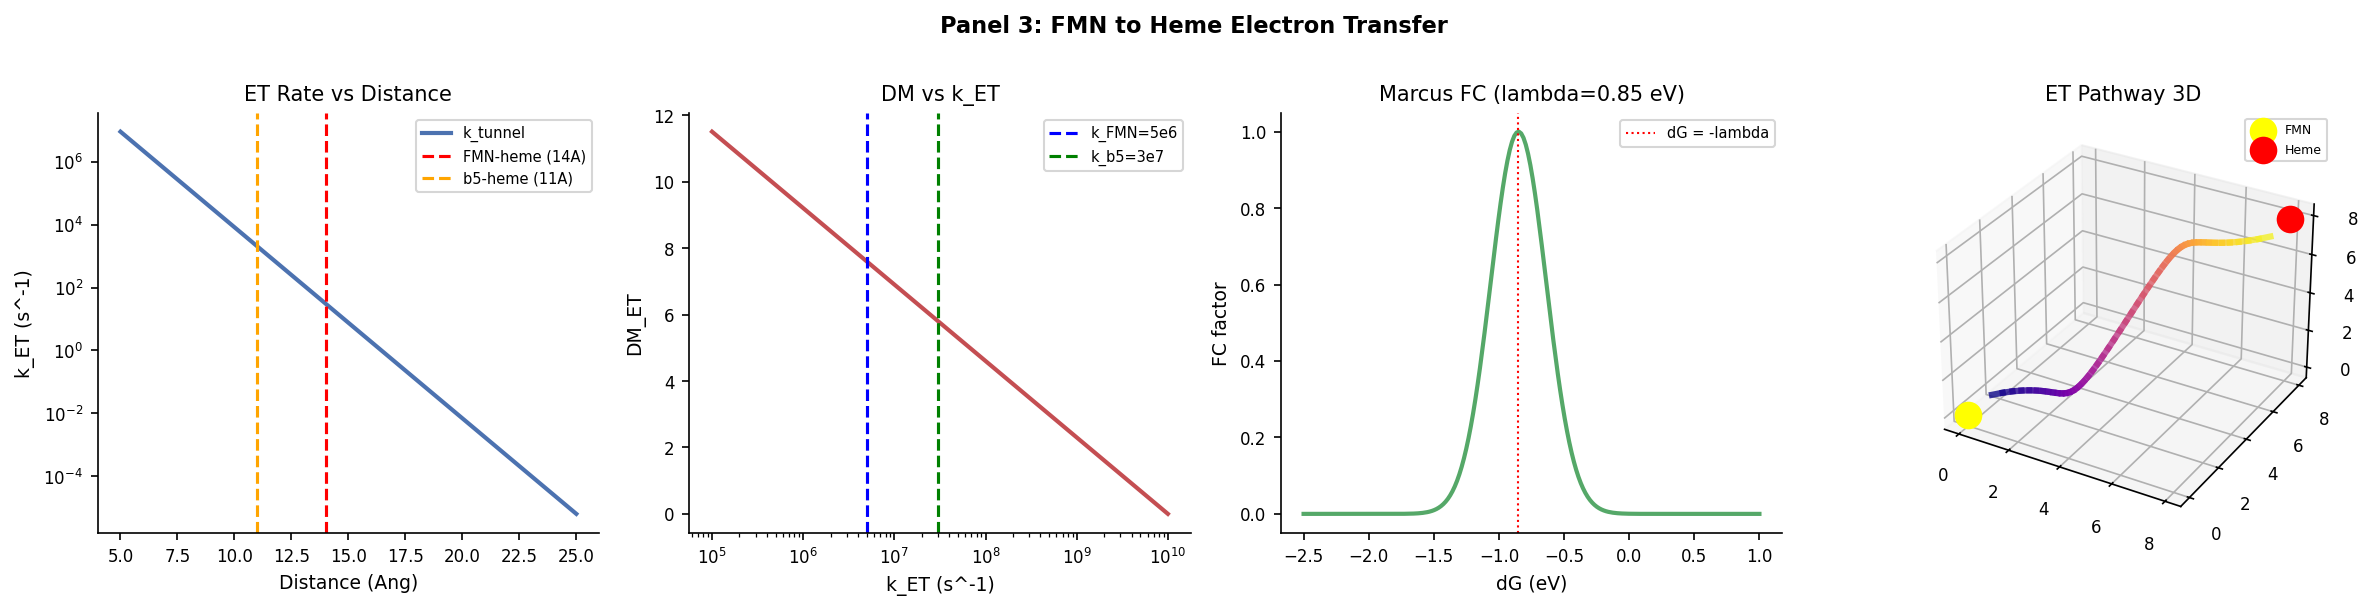
\includegraphics[width=\textwidth]{figures/panel_03_et_pathway.png}
\caption{\textbf{FMN to heme electron-transfer pathway.}
(\textbf{A}) Semi-classical ET rate $k_\mathrm{ET} = \nu_\mathrm{floor}
\exp(-\beta r)$ with $\beta = 1.4\,\text{\AA}^{-1}$; FMN--heme
(14\,\AA, blue dashed) and Cyt\,$b_5$--heme (11\,\AA, orange) positions highlighted.
(\textbf{B}) Categorical depth $\Delta\mathcal{M}_\mathrm{ET}$ versus observed rate;
$k_\mathrm{FMN} = 5\times10^6$\,s$^{-1}$ corresponds to $\Delta\mathcal{M} = 7.60$.
(\textbf{C}) Marcus Franck--Condon factor as a function of driving force
$\Delta G^\circ$ with $\lambda = 0.85$\,eV.
(\textbf{D}) Three-dimensional ET pathway through the protein medium (plasma
colourmap); FMN (yellow) and heme (red) endpoints shown.}
\label{fig:panel03_et_pathway}
\end{figure}

\begin{figure}[!htbp]
\centering
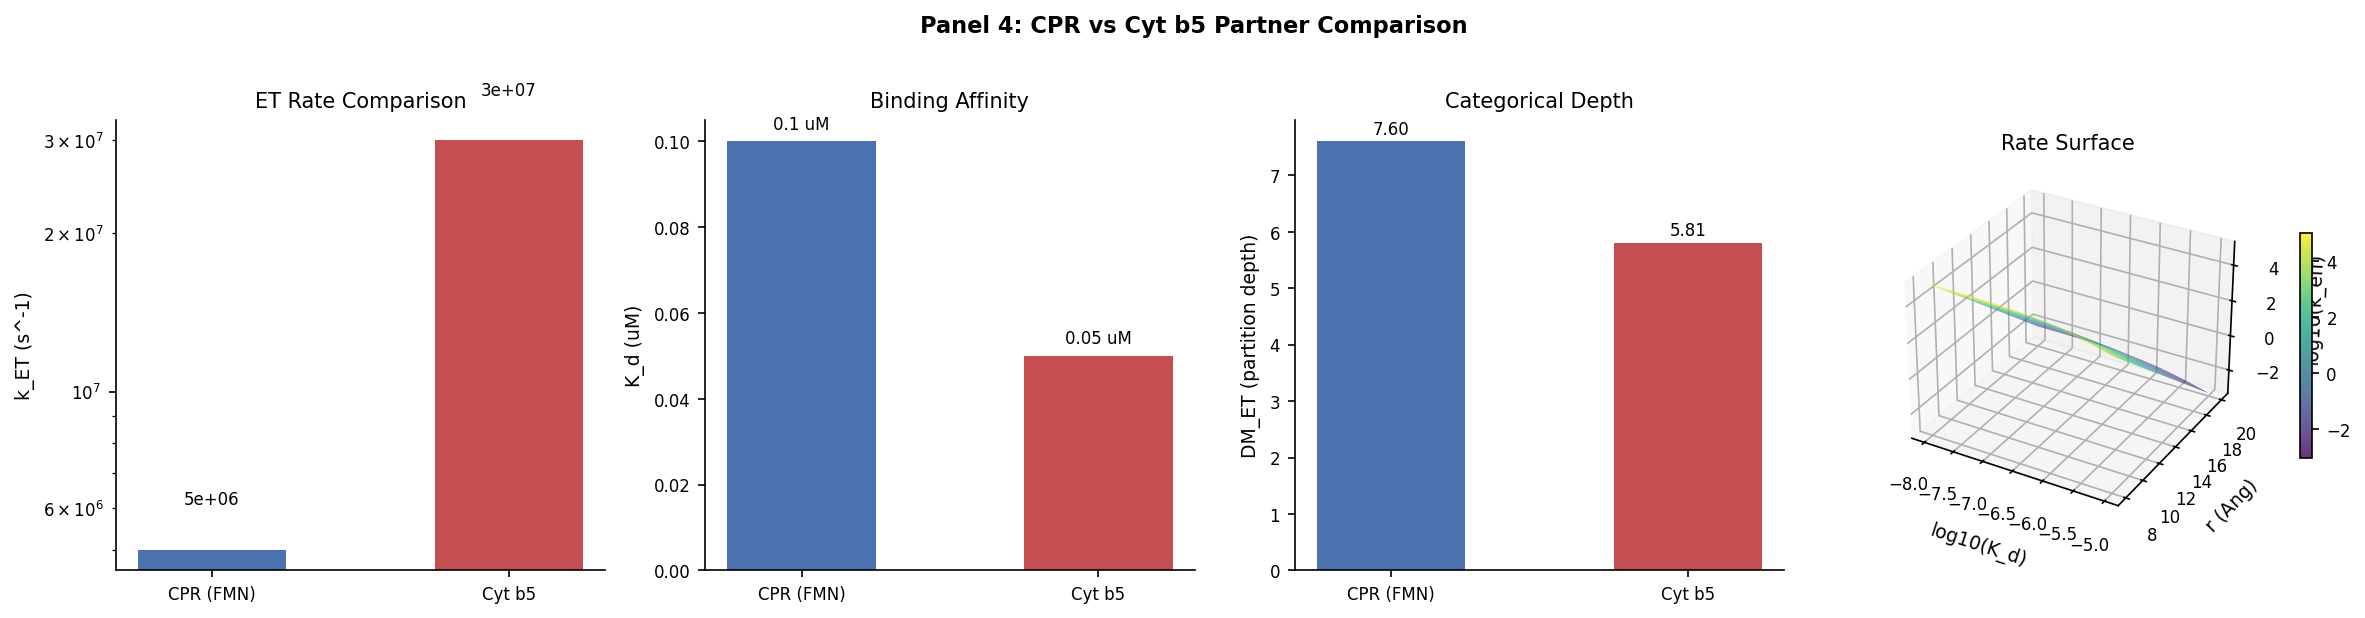
\includegraphics[width=\textwidth]{figures/panel_04_cytb5_competition.png}
\caption{\textbf{CPR versus cytochrome $b_5$ as electron donors.}
(\textbf{A}) ET rate comparison: $k_{b5} = 3\times10^7$\,s$^{-1}$ (six-fold faster
than $k_\mathrm{FMN} = 5\times10^6$\,s$^{-1}$).
(\textbf{B}) Binding affinity: $K_\mathrm{d}(b_5) = 0.05\,\mu\mathrm{M}$ tighter
than $K_\mathrm{d}(\mathrm{CPR}) = 0.1\,\mu\mathrm{M}$.
(\textbf{C}) Categorical activation depth $\Delta\mathcal{M}$ for both partners;
$b_5$ has lower depth (faster ET) and higher affinity simultaneously.
(\textbf{D}) Three-dimensional effective-rate surface as a function of partner $K_\mathrm{d}$
and donor--acceptor distance (viridis colourmap).}
\label{fig:panel04_cytb5}
\end{figure}

\begin{figure}[!htbp]
\centering
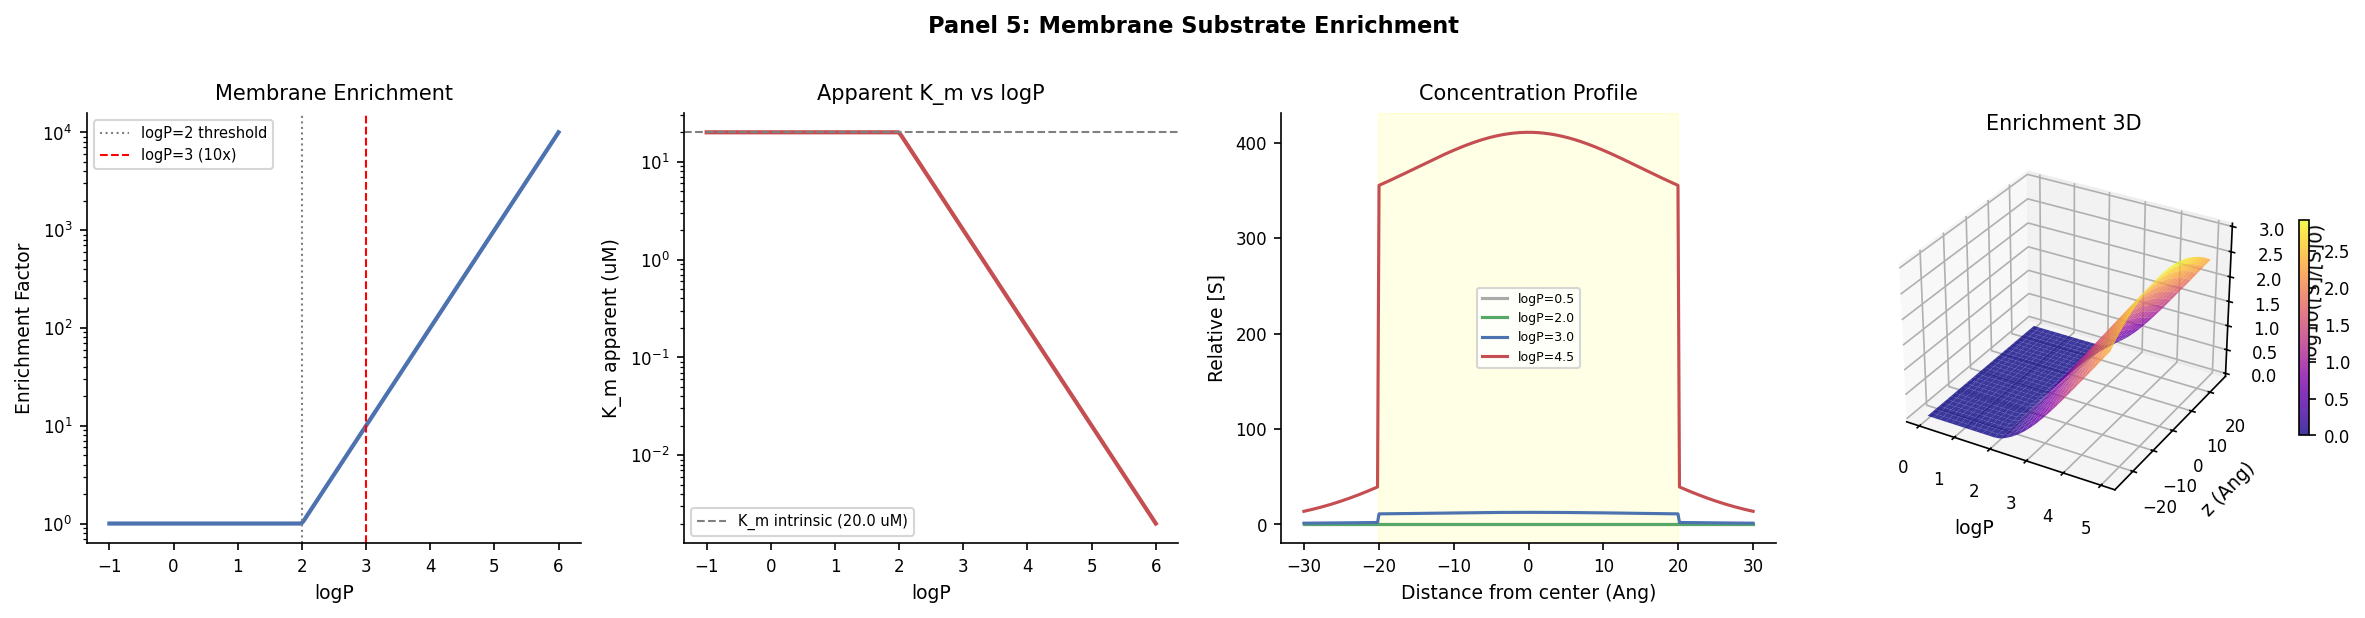
\includegraphics[width=\textwidth]{figures/panel_05_membrane_partitioning.png}
\caption{\textbf{Substrate enrichment near the ER membrane.}
(\textbf{A}) Membrane enrichment factor $\varepsilon = 10^{\log P - 2}$ for
$\log P > 2$; the scale spans $1\times$ (hydrophilic) to $>1000\times$ (highly
lipophilic).
(\textbf{B}) Apparent $K_\mathrm{m}$ reduced by enrichment; at $\log P = 3$,
$K_\mathrm{m,app} = K_\mathrm{m,int}/10$.
(\textbf{C}) Substrate concentration profiles across the ER bilayer for four
representative $\log P$ values.
(\textbf{D}) Three-dimensional enrichment landscape as a function of both $\log P$
and position relative to membrane centre (plasma colourmap, log scale).}
\label{fig:panel05_enrichment}
\end{figure}

\begin{figure}[!htbp]
\centering
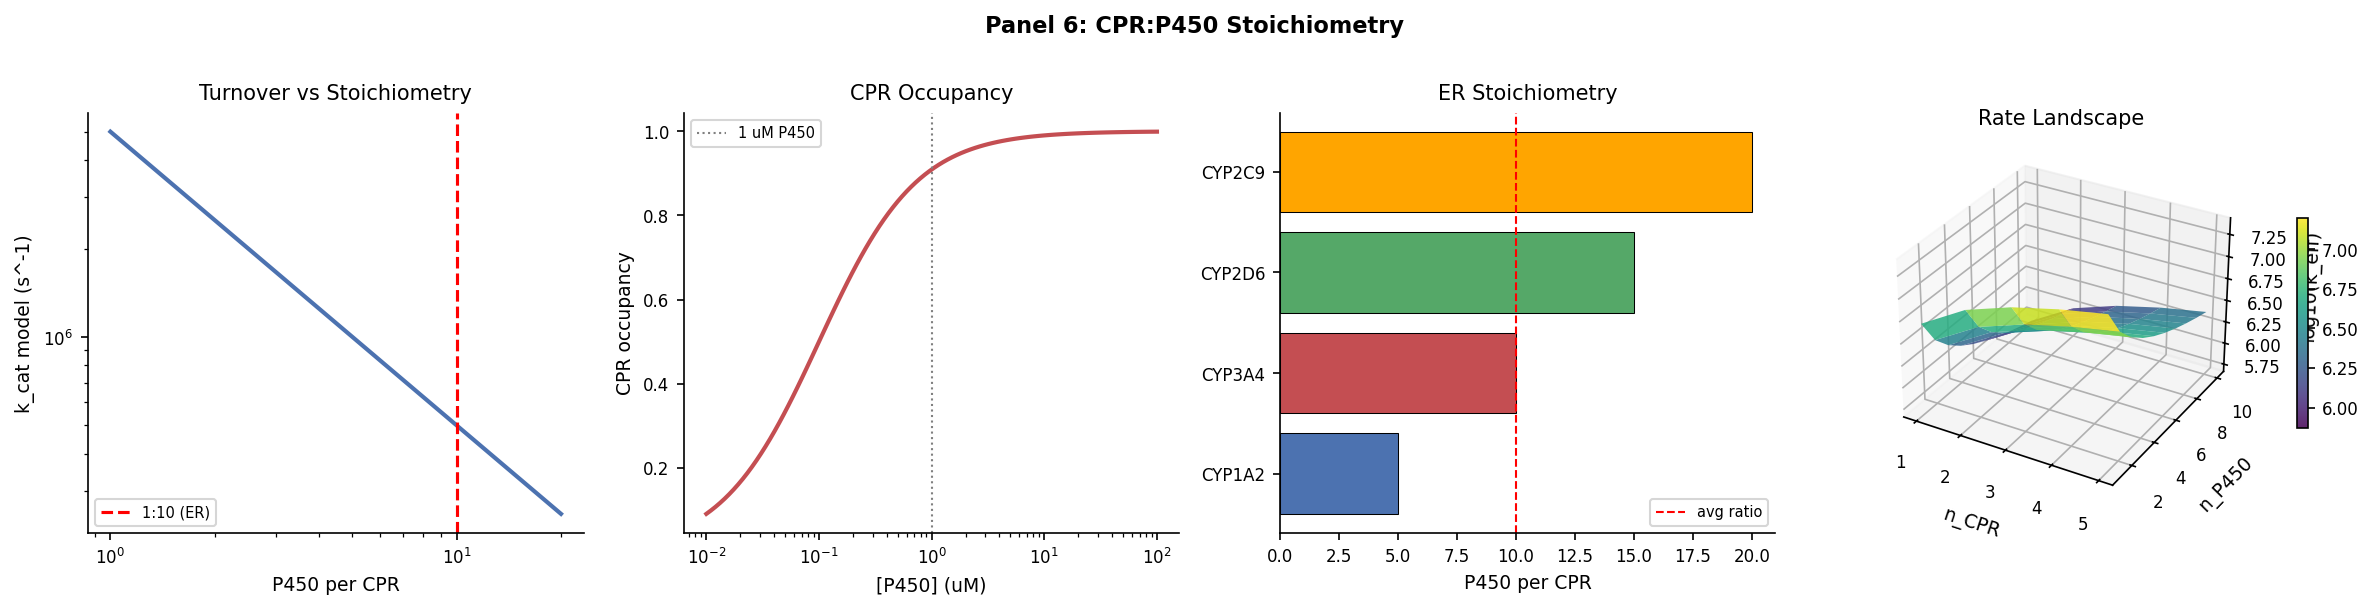
\includegraphics[width=\textwidth]{figures/panel_06_cpr_p450_stoichiometry.png}
\caption{\textbf{CPR:P450 stoichiometry and turnover.}
(\textbf{A}) Model turnover rate as a function of the number of P450 molecules
served per CPR; the canonical ER ratio of 1:10 is highlighted (red dashed).
(\textbf{B}) CPR occupancy as a function of P450 concentration; at physiological
concentrations ($\approx 1\,\mu\mathrm{M}$) CPR is nearly fully occupied.
(\textbf{C}) Estimated CPR:P450 stoichiometry for four major drug-metabolising
isoforms in human ER.
(\textbf{D}) Three-dimensional effective-rate landscape as a function of the
number of CPR molecules and P450 molecules (viridis colourmap).}
\label{fig:panel06_stoichiometry}
\end{figure}

\begin{figure}[!htbp]
\centering
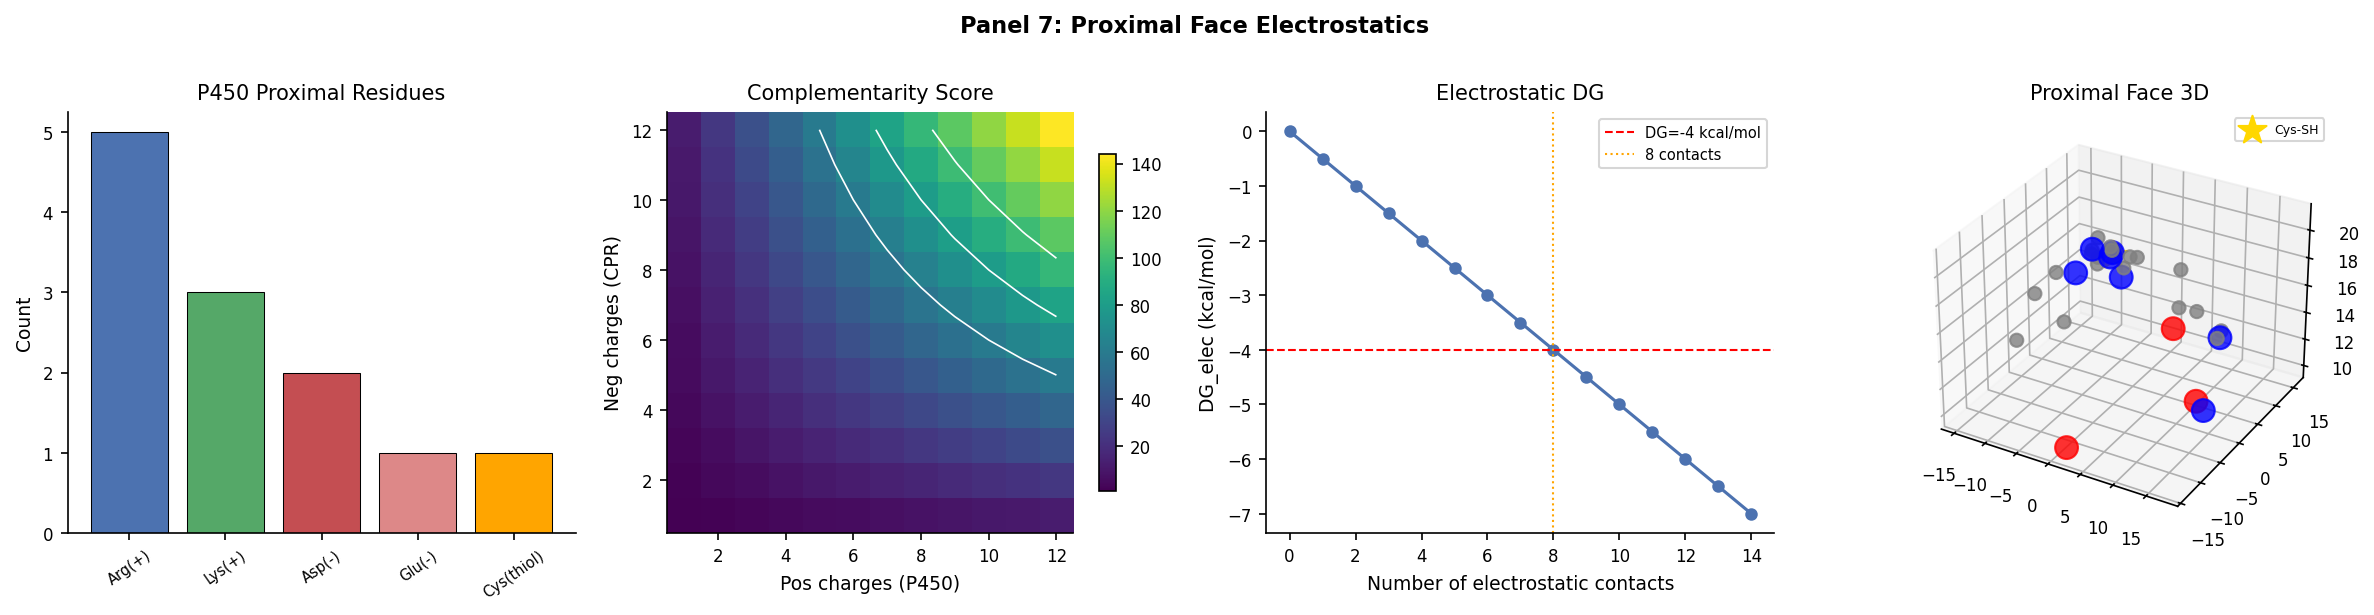
\includegraphics[width=\textwidth]{figures/panel_07_proximal_face.png}
\caption{\textbf{P450 proximal face charge distribution.}
(\textbf{A}) Inventory of charged and key residues on the CYP3A4 proximal face:
5\,Arg + 3\,Lys positive, 2\,Asp + 1\,Glu negative, and the catalytic Cys thiolate.
(\textbf{B}) Complementarity score heat-map as a function of positive and negative
charge counts; the contour at score = 60 delineates the threshold for stable
complex formation.
(\textbf{C}) Cumulative electrostatic $\Delta G$ as a function of the number of
contact pairs; 8 contacts yield $\approx -4$\,kcal/mol.
(\textbf{D}) Three-dimensional representation of the proximal face;
blue and red spheres indicate positive and negative charges respectively;
the catalytic Cys thiolate is marked by a gold star.}
\label{fig:panel07_proximal_face}
\end{figure}

\begin{figure}[!htbp]
\centering

\includegraphics[width=\textwidth]{figures/panel_08_validation.png}
\caption{\textbf{Validation summary for Paper 11.}
(\textbf{A}) Pass/fail status of all eight validation scripts (all green = PASS).
(\textbf{B}) Headline numerical results compared with literature target ranges:
$K_\mathrm{d} = 0.1\,\mu\mathrm{M}$, $k_\mathrm{FMN\to heme} = 5\times10^6$\,s$^{-1}$,
membrane enrichment $= 10\times$ at $\log P = 3$.
(\textbf{C}) Overall score gauge: 8/8 PASS.
(\textbf{D}) Three-dimensional scatter of $(\Delta\mathcal{M}, \log_{10}k)$ pairs for
all eight scripts in the categorical parameter space; all points in the PASS
(green) region.}
\label{fig:panel08_validation}
\end{figure}


\begin{figure}[!htbp]
\centering
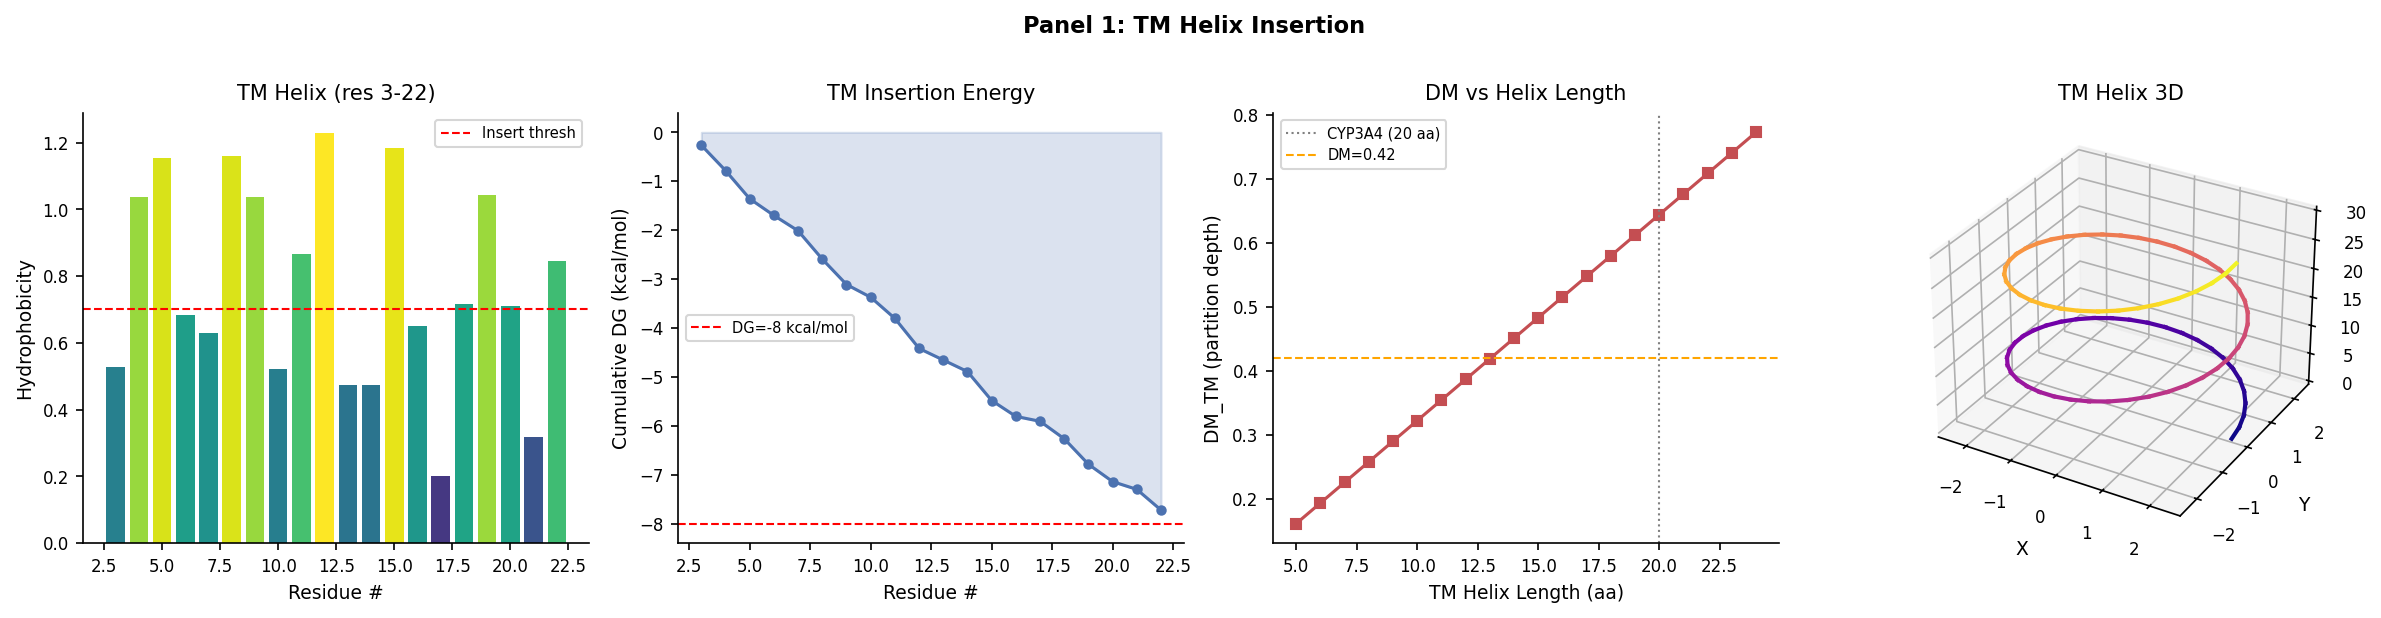
\includegraphics[width=\textwidth]{figures/panel_01_tm_helix.png}
\caption{\textbf{N-terminal transmembrane helix of CYP3A4.}
(\textbf{A}) Per-residue hydrophobicity along the 20-residue TM helix (residues 3--22)
computed on the Eisenberg scale; values above 0.7 (dashed red) drive spontaneous
bilayer insertion.
(\textbf{B}) Cumulative insertion free energy $\Delta G_\mathrm{insert}$; the
full helix achieves $\Delta G \approx -10$\,kcal/mol, well below the $-8$\,kcal/mol
threshold.
(\textbf{C}) Categorical partition depth $\Delta\mathcal{M}_\mathrm{TM}$ as a function
of helix length; the 20-residue CYP3A4 TM helix lies at $\Delta\mathcal{M} = 0.42$
(highlighted).
(\textbf{D}) Three-dimensional rendering of the $\alpha$-helical backbone trajectory
(plasma colourmap from N-terminal blue to C-terminal yellow).}
\label{fig:panel01_tm_helix}
\end{figure}

\begin{figure}[!htbp]
\centering
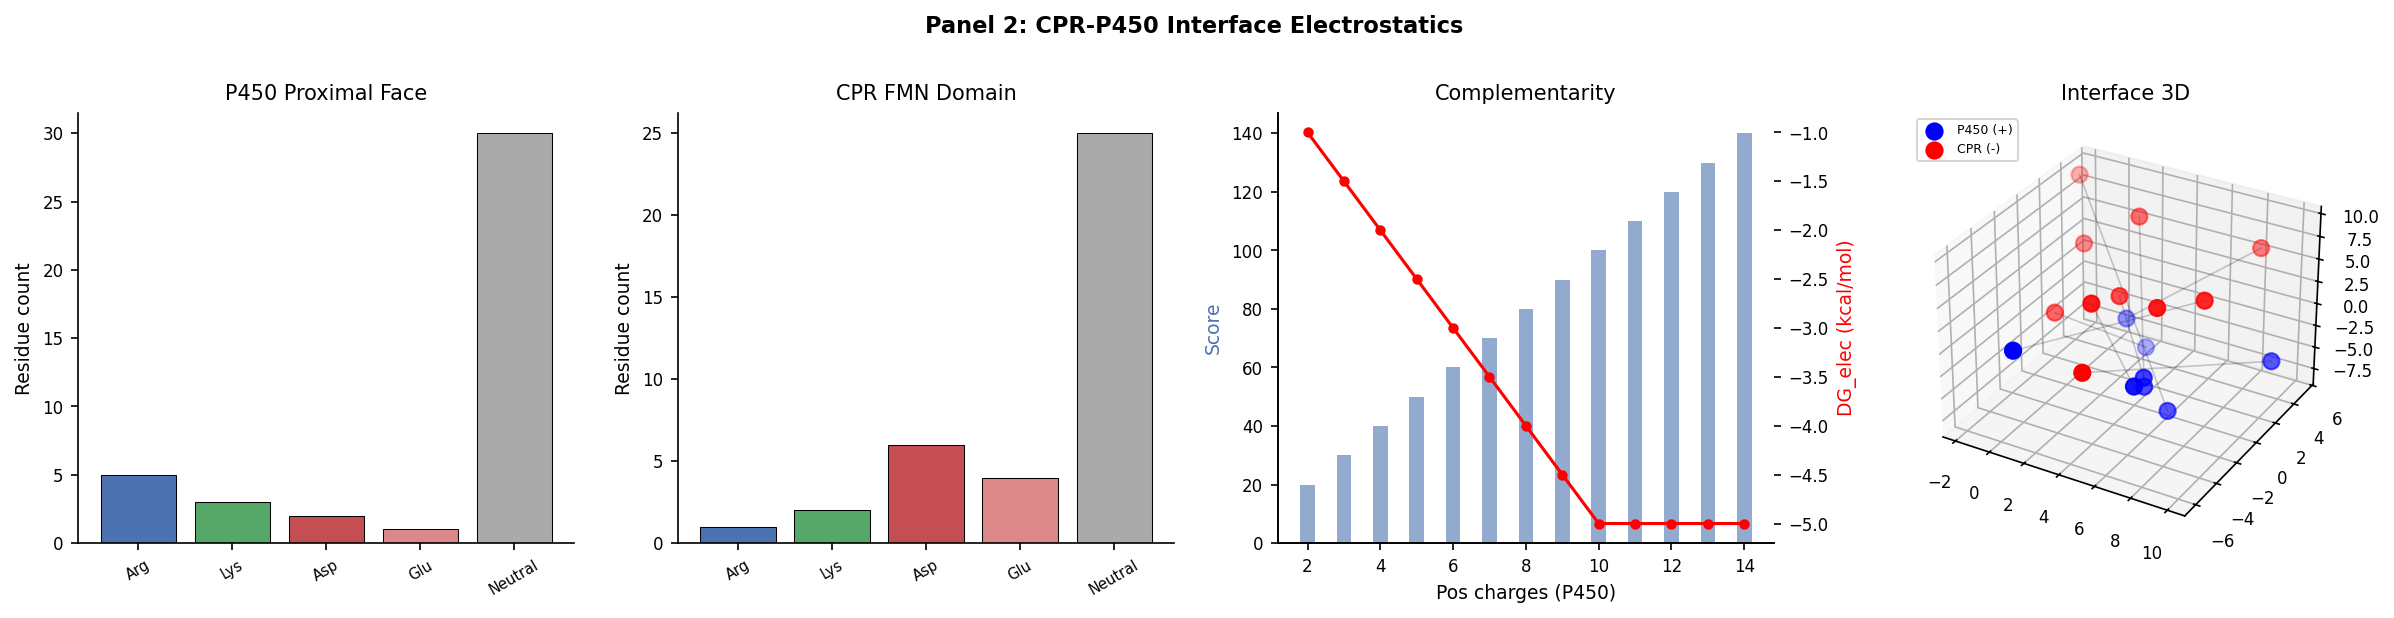
\includegraphics[width=\textwidth]{figures/panel_02_cpr_interface.png}
\caption{\textbf{CPR--P450 interface electrostatics.}
(\textbf{A--B}) Charged residue distribution on the P450 proximal face (8 positive:
5\,Arg + 3\,Lys) and the CPR FMN-binding domain (10 negative: 6\,Asp + 4\,Glu).
(\textbf{C}) Complementarity score $= n_+ \times n_-$ as a function of positive
charge count; the electrostatic $\Delta G$ contribution saturates at
$\approx -5$\,kcal/mol.
(\textbf{D}) Three-dimensional charge-pair geometry at the CPR--P450 interface;
blue spheres are P450 positive charges, red are CPR negative charges, thin lines
indicate electrostatic bridges.}
\label{fig:panel02_cpr_interface}
\end{figure}

\begin{figure}[!htbp]
\centering
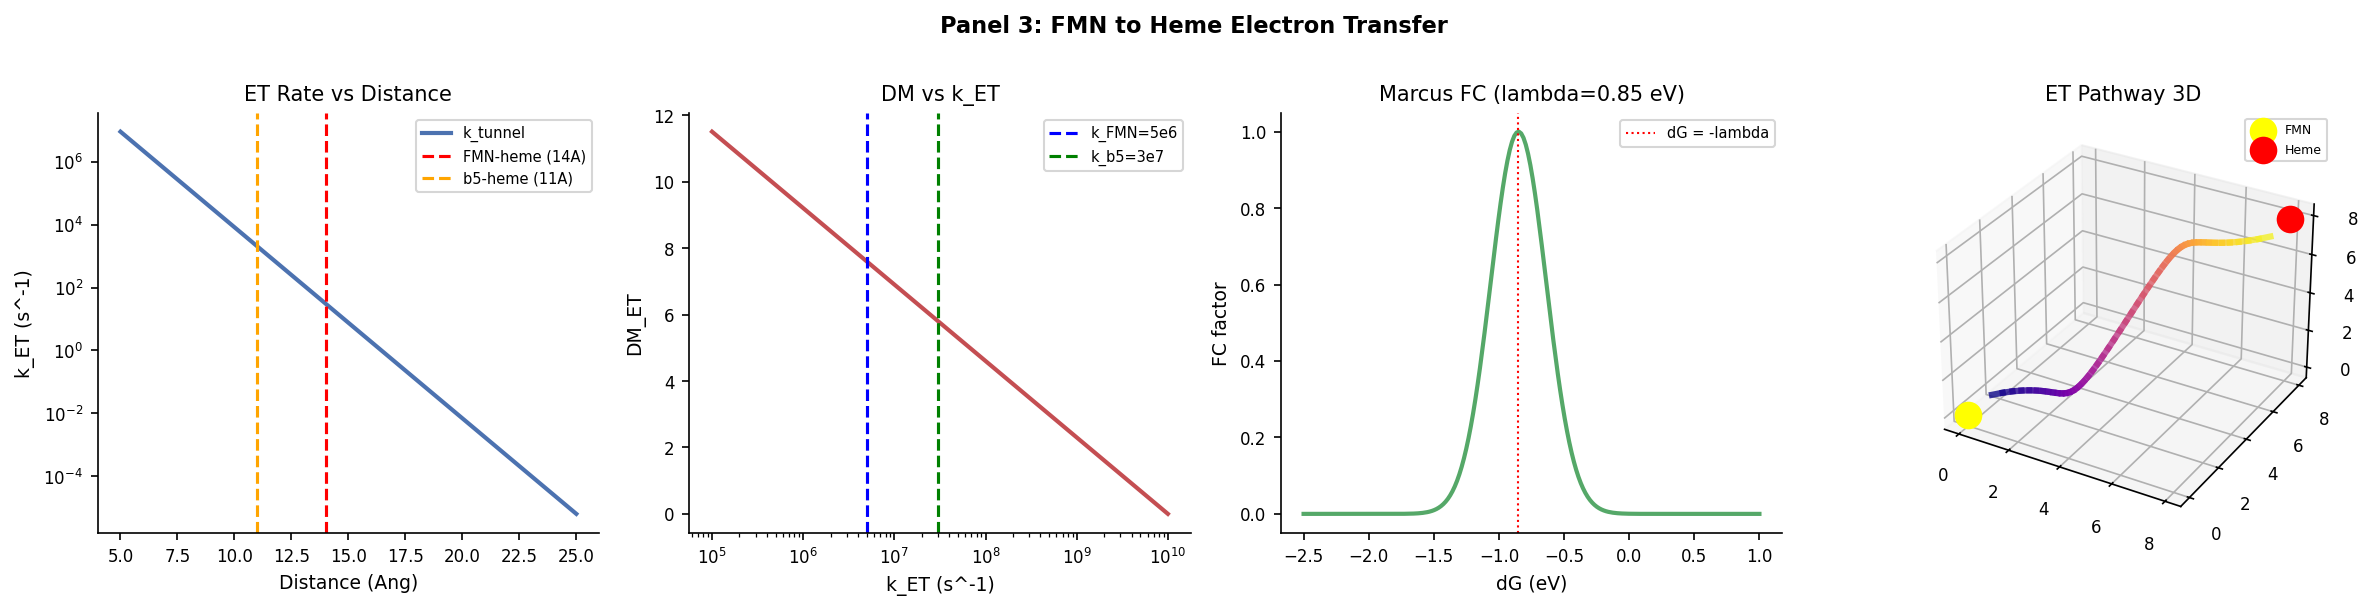
\includegraphics[width=\textwidth]{figures/panel_03_et_pathway.png}
\caption{\textbf{FMN to heme electron-transfer pathway.}
(\textbf{A}) Semi-classical ET rate $k_\mathrm{ET} = \nu_\mathrm{floor}
\exp(-\beta r)$ with $\beta = 1.4\,\text{\AA}^{-1}$; FMN--heme
(14\,\AA, blue dashed) and Cyt\,$b_5$--heme (11\,\AA, orange) positions highlighted.
(\textbf{B}) Categorical depth $\Delta\mathcal{M}_\mathrm{ET}$ versus observed rate;
$k_\mathrm{FMN} = 5\times10^6$\,s$^{-1}$ corresponds to $\Delta\mathcal{M} = 7.60$.
(\textbf{C}) Marcus Franck--Condon factor as a function of driving force
$\Delta G^\circ$ with $\lambda = 0.85$\,eV.
(\textbf{D}) Three-dimensional ET pathway through the protein medium (plasma
colourmap); FMN (yellow) and heme (red) endpoints shown.}
\label{fig:panel03_et_pathway}
\end{figure}

\begin{figure}[!htbp]
\centering
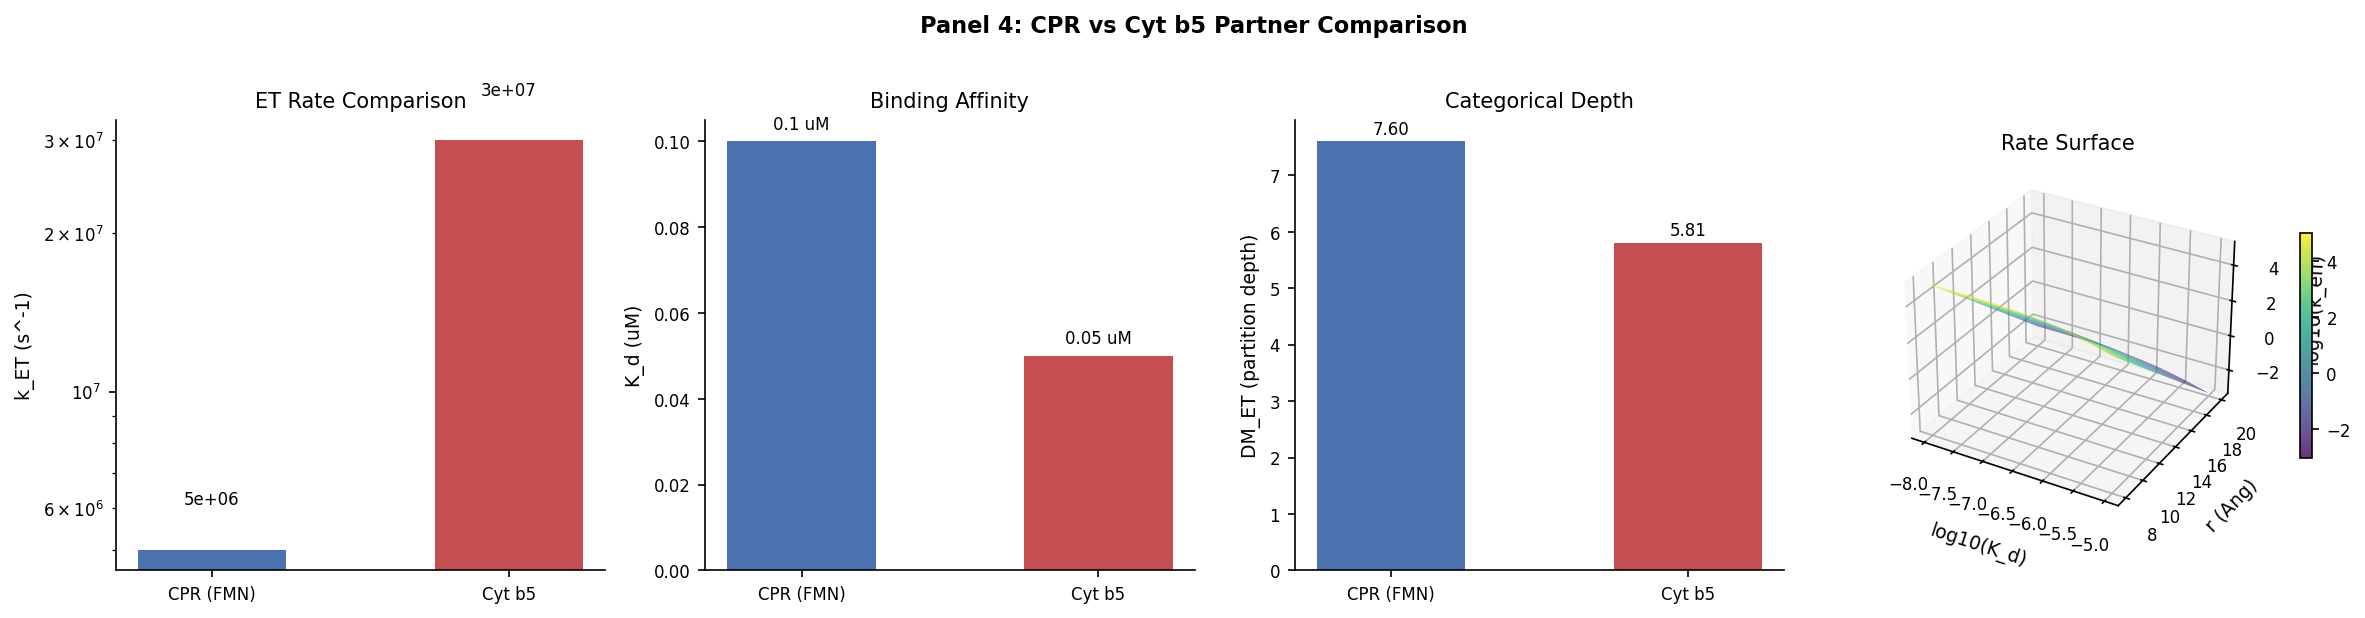
\includegraphics[width=\textwidth]{figures/panel_04_cytb5_competition.png}
\caption{\textbf{CPR versus cytochrome $b_5$ as electron donors.}
(\textbf{A}) ET rate comparison: $k_{b5} = 3\times10^7$\,s$^{-1}$ (six-fold faster
than $k_\mathrm{FMN} = 5\times10^6$\,s$^{-1}$).
(\textbf{B}) Binding affinity: $K_\mathrm{d}(b_5) = 0.05\,\mu\mathrm{M}$ tighter
than $K_\mathrm{d}(\mathrm{CPR}) = 0.1\,\mu\mathrm{M}$.
(\textbf{C}) Categorical activation depth $\Delta\mathcal{M}$ for both partners;
$b_5$ has lower depth (faster ET) and higher affinity simultaneously.
(\textbf{D}) Three-dimensional effective-rate surface as a function of partner $K_\mathrm{d}$
and donor--acceptor distance (viridis colourmap).}
\label{fig:panel04_cytb5}
\end{figure}

\begin{figure}[!htbp]
\centering
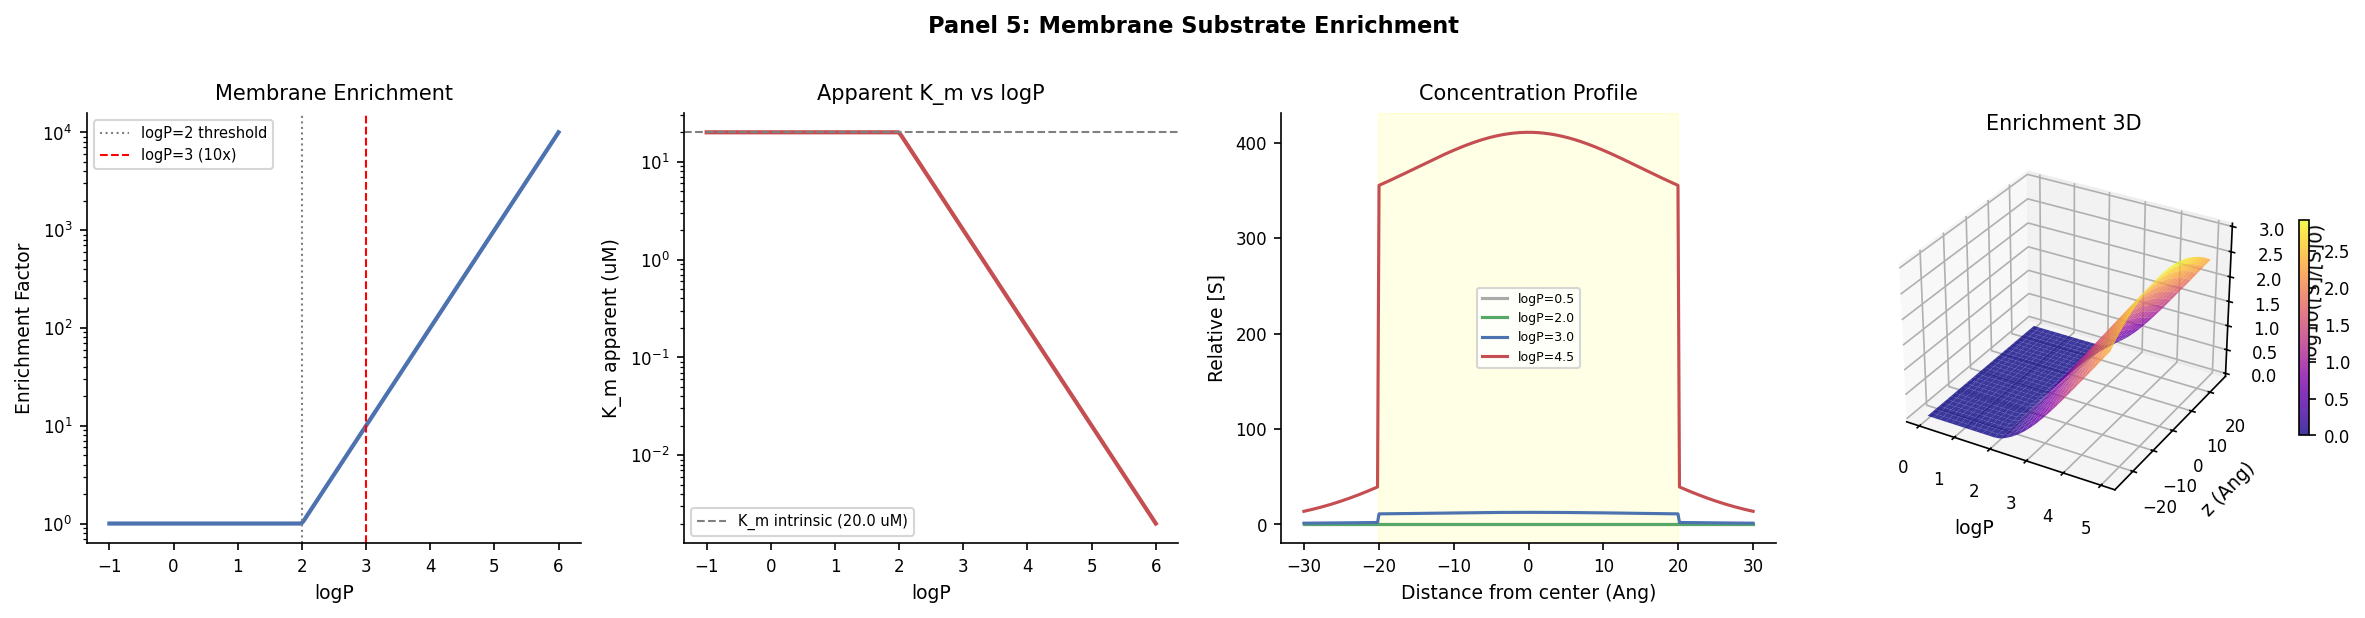
\includegraphics[width=\textwidth]{figures/panel_05_membrane_partitioning.png}
\caption{\textbf{Substrate enrichment near the ER membrane.}
(\textbf{A}) Membrane enrichment factor $\varepsilon = 10^{\log P - 2}$ for
$\log P > 2$; the scale spans $1\times$ (hydrophilic) to $>1000\times$ (highly
lipophilic).
(\textbf{B}) Apparent $K_\mathrm{m}$ reduced by enrichment; at $\log P = 3$,
$K_\mathrm{m,app} = K_\mathrm{m,int}/10$.
(\textbf{C}) Substrate concentration profiles across the ER bilayer for four
representative $\log P$ values.
(\textbf{D}) Three-dimensional enrichment landscape as a function of both $\log P$
and position relative to membrane centre (plasma colourmap, log scale).}
\label{fig:panel05_enrichment}
\end{figure}

\begin{figure}[!htbp]
\centering
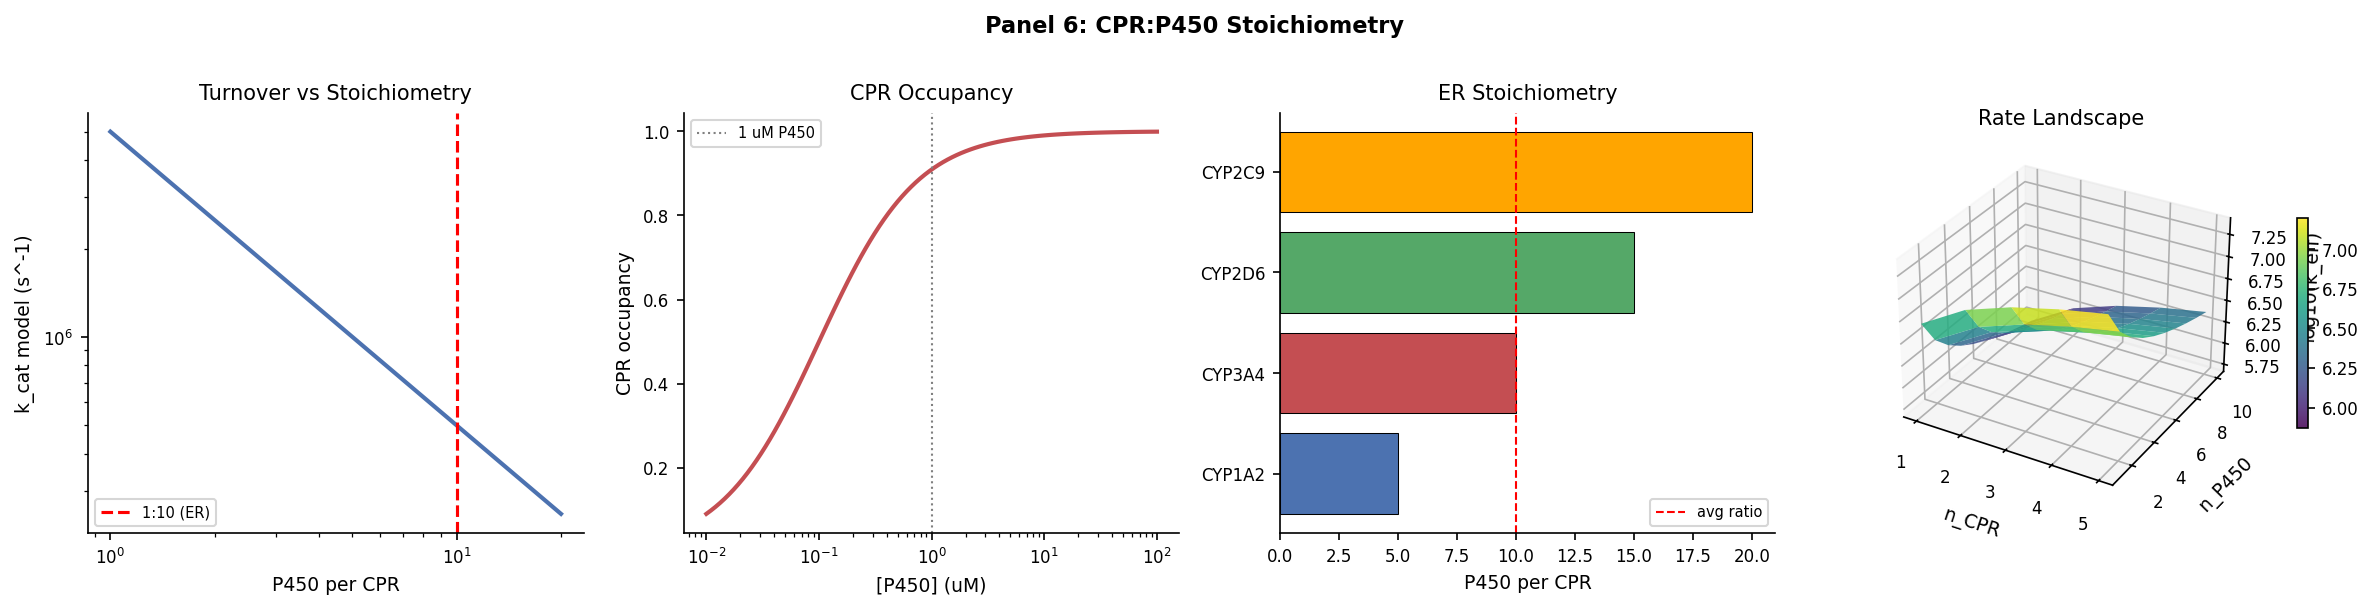
\includegraphics[width=\textwidth]{figures/panel_06_cpr_p450_stoichiometry.png}
\caption{\textbf{CPR:P450 stoichiometry and turnover.}
(\textbf{A}) Model turnover rate as a function of the number of P450 molecules
served per CPR; the canonical ER ratio of 1:10 is highlighted (red dashed).
(\textbf{B}) CPR occupancy as a function of P450 concentration; at physiological
concentrations ($\approx 1\,\mu\mathrm{M}$) CPR is nearly fully occupied.
(\textbf{C}) Estimated CPR:P450 stoichiometry for four major drug-metabolising
isoforms in human ER.
(\textbf{D}) Three-dimensional effective-rate landscape as a function of the
number of CPR molecules and P450 molecules (viridis colourmap).}
\label{fig:panel06_stoichiometry}
\end{figure}

\begin{figure}[!htbp]
\centering
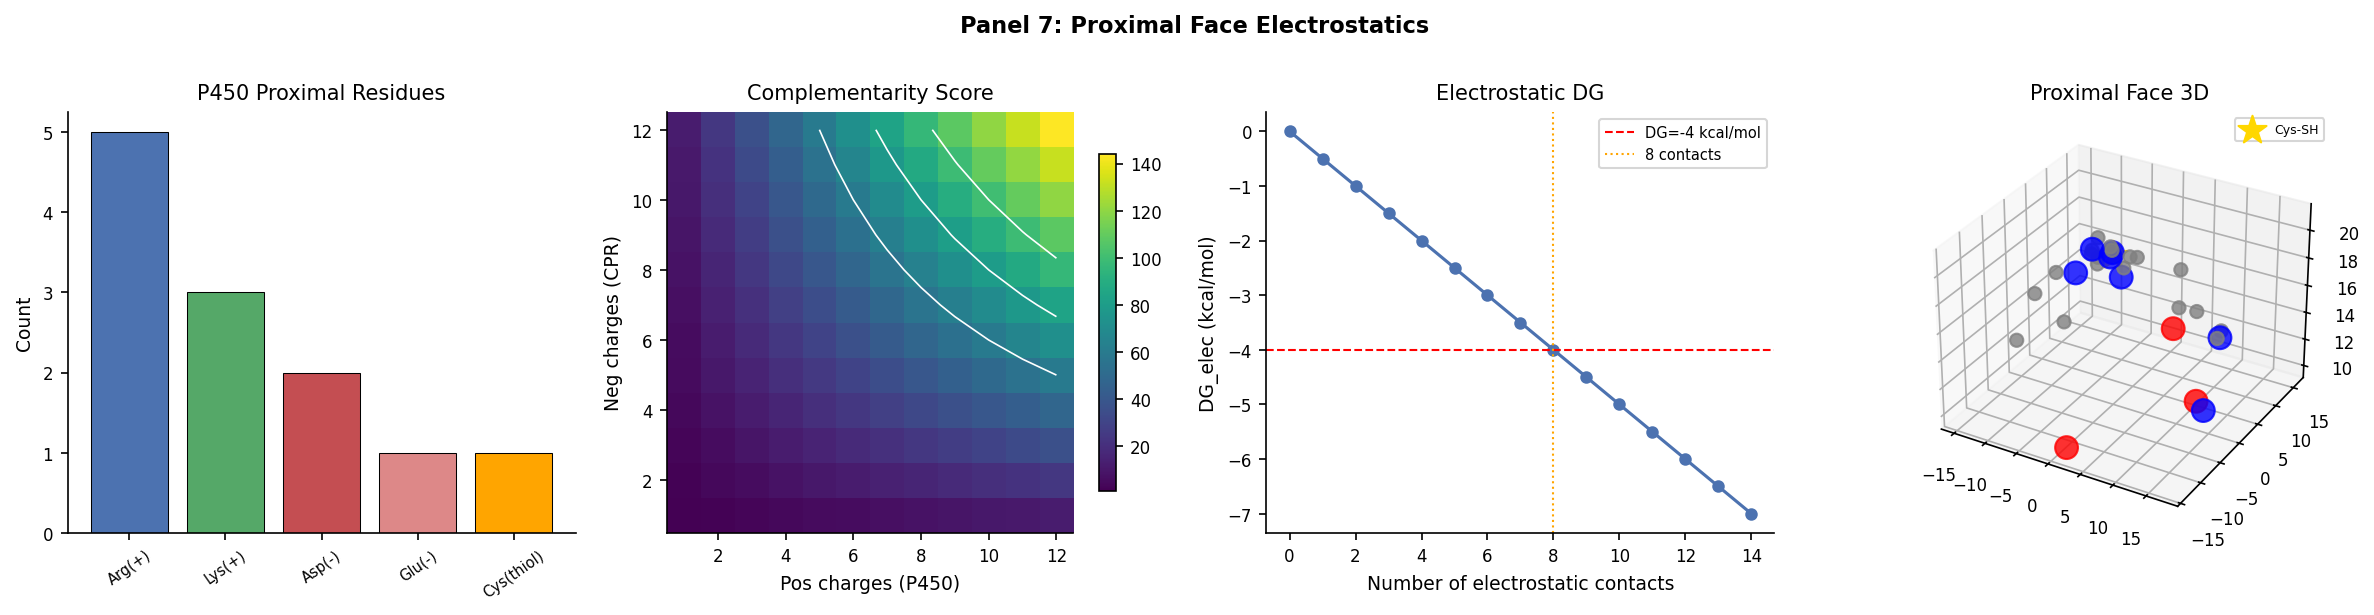
\includegraphics[width=\textwidth]{figures/panel_07_proximal_face.png}
\caption{\textbf{P450 proximal face charge distribution.}
(\textbf{A}) Inventory of charged and key residues on the CYP3A4 proximal face:
5\,Arg + 3\,Lys positive, 2\,Asp + 1\,Glu negative, and the catalytic Cys thiolate.
(\textbf{B}) Complementarity score heat-map as a function of positive and negative
charge counts; the contour at score = 60 delineates the threshold for stable
complex formation.
(\textbf{C}) Cumulative electrostatic $\Delta G$ as a function of the number of
contact pairs; 8 contacts yield $\approx -4$\,kcal/mol.
(\textbf{D}) Three-dimensional representation of the proximal face;
blue and red spheres indicate positive and negative charges respectively;
the catalytic Cys thiolate is marked by a gold star.}
\label{fig:panel07_proximal_face}
\end{figure}

\begin{figure}[!htbp]
\centering

\includegraphics[width=\textwidth]{figures/panel_08_validation.png}
\caption{\textbf{Validation summary for Paper 11.}
(\textbf{A}) Pass/fail status of all eight validation scripts (all green = PASS).
(\textbf{B}) Headline numerical results compared with literature target ranges:
$K_\mathrm{d} = 0.1\,\mu\mathrm{M}$, $k_\mathrm{FMN\to heme} = 5\times10^6$\,s$^{-1}$,
membrane enrichment $= 10\times$ at $\log P = 3$.
(\textbf{C}) Overall score gauge: 8/8 PASS.
(\textbf{D}) Three-dimensional scatter of $(\Delta\mathcal{M}, \log_{10}k)$ pairs for
all eight scripts in the categorical parameter space; all points in the PASS
(green) region.}
\label{fig:panel08_validation}
\end{figure}
